This section will analyze and discuss the results obtained in this study. 
The main objective is to understand the energy consumed by different DBMS.
 We will try to understand how the CPU and secondary storage energy consumption and to try to related to the performance of which DBMS. Additionally, we want to understand the impact of different environments (number of users) on energy consumption on which DBMS.
 \subsection{Results}
 
 
%% MEDIANS

\begin{figure*}[h]
\centering
\caption{Median of energy consumption on Package , Disk and Total.}
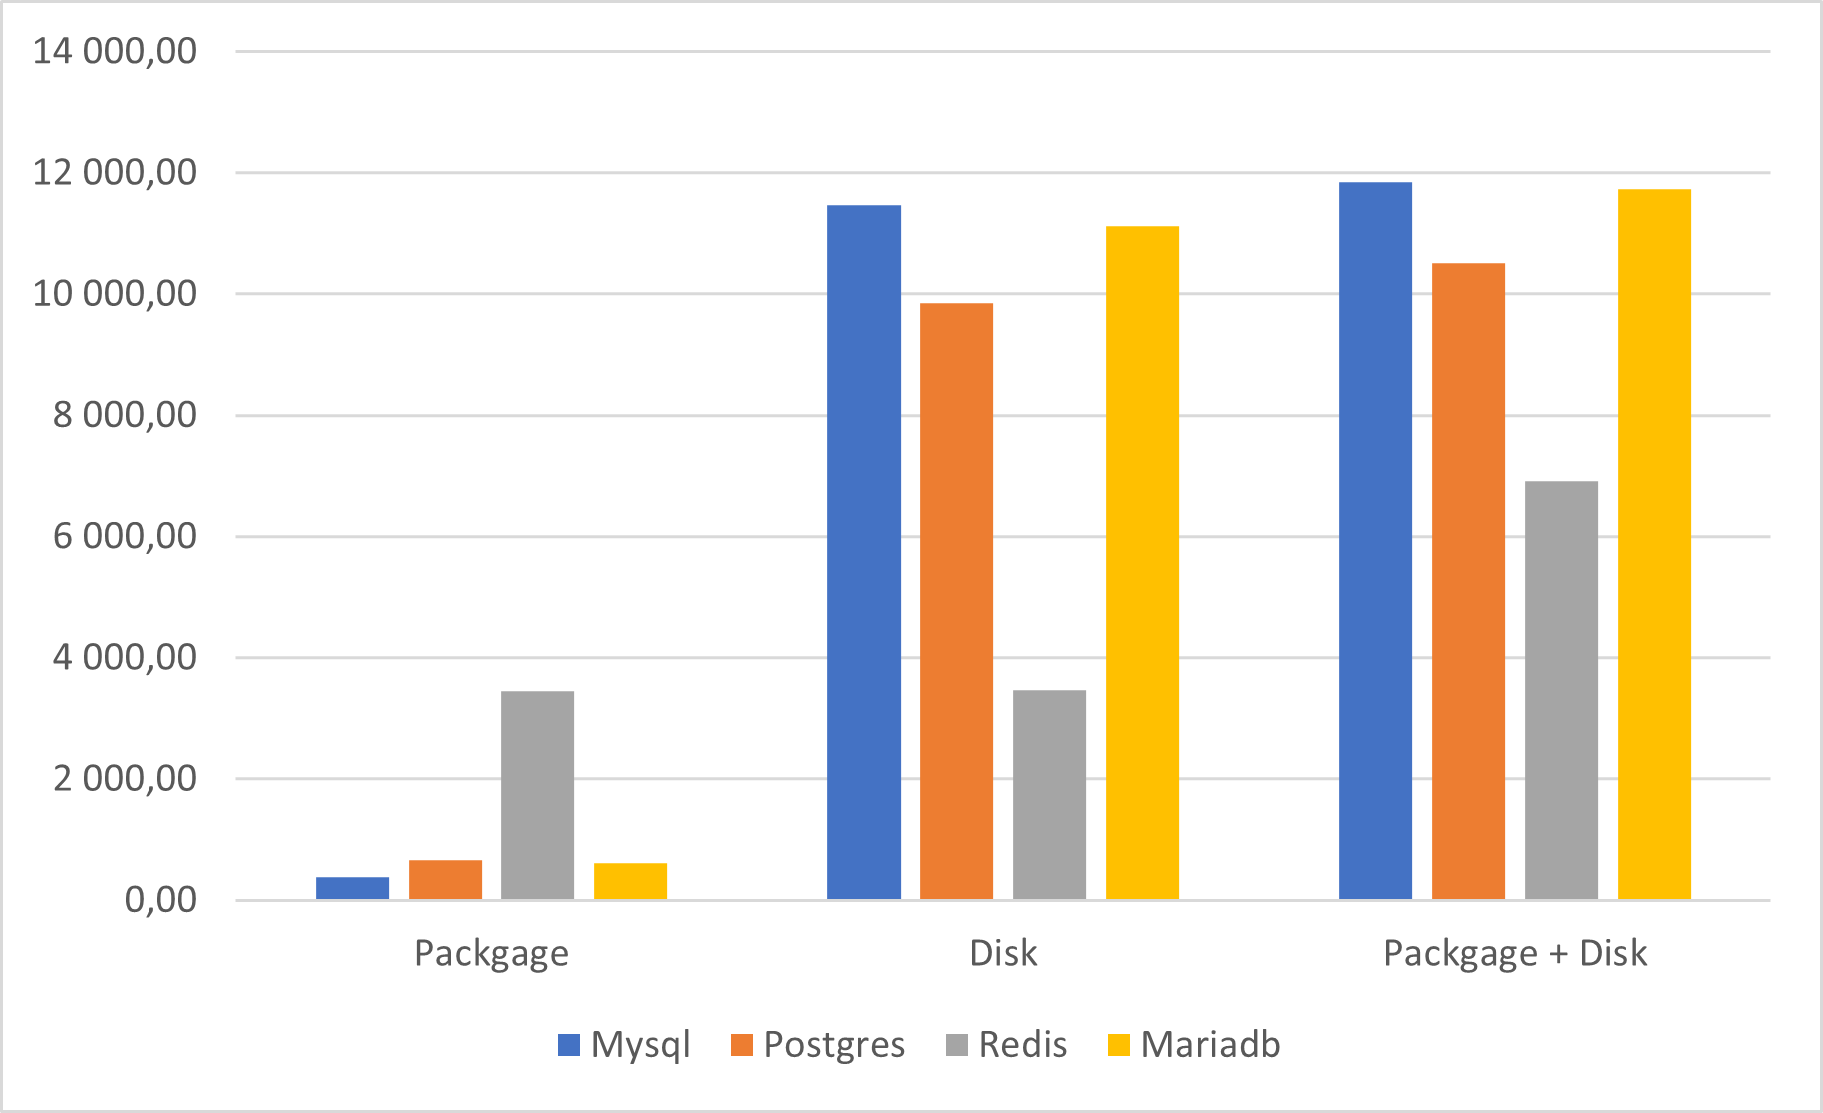
\includegraphics[width=0.6\columnwidth]{results/median/energy.png}
\label{fig:medianenergy}
\end{figure*}

\begin{figure*}[h]
\centering
\caption{Median of Transitions per minute and New orders per minute.}
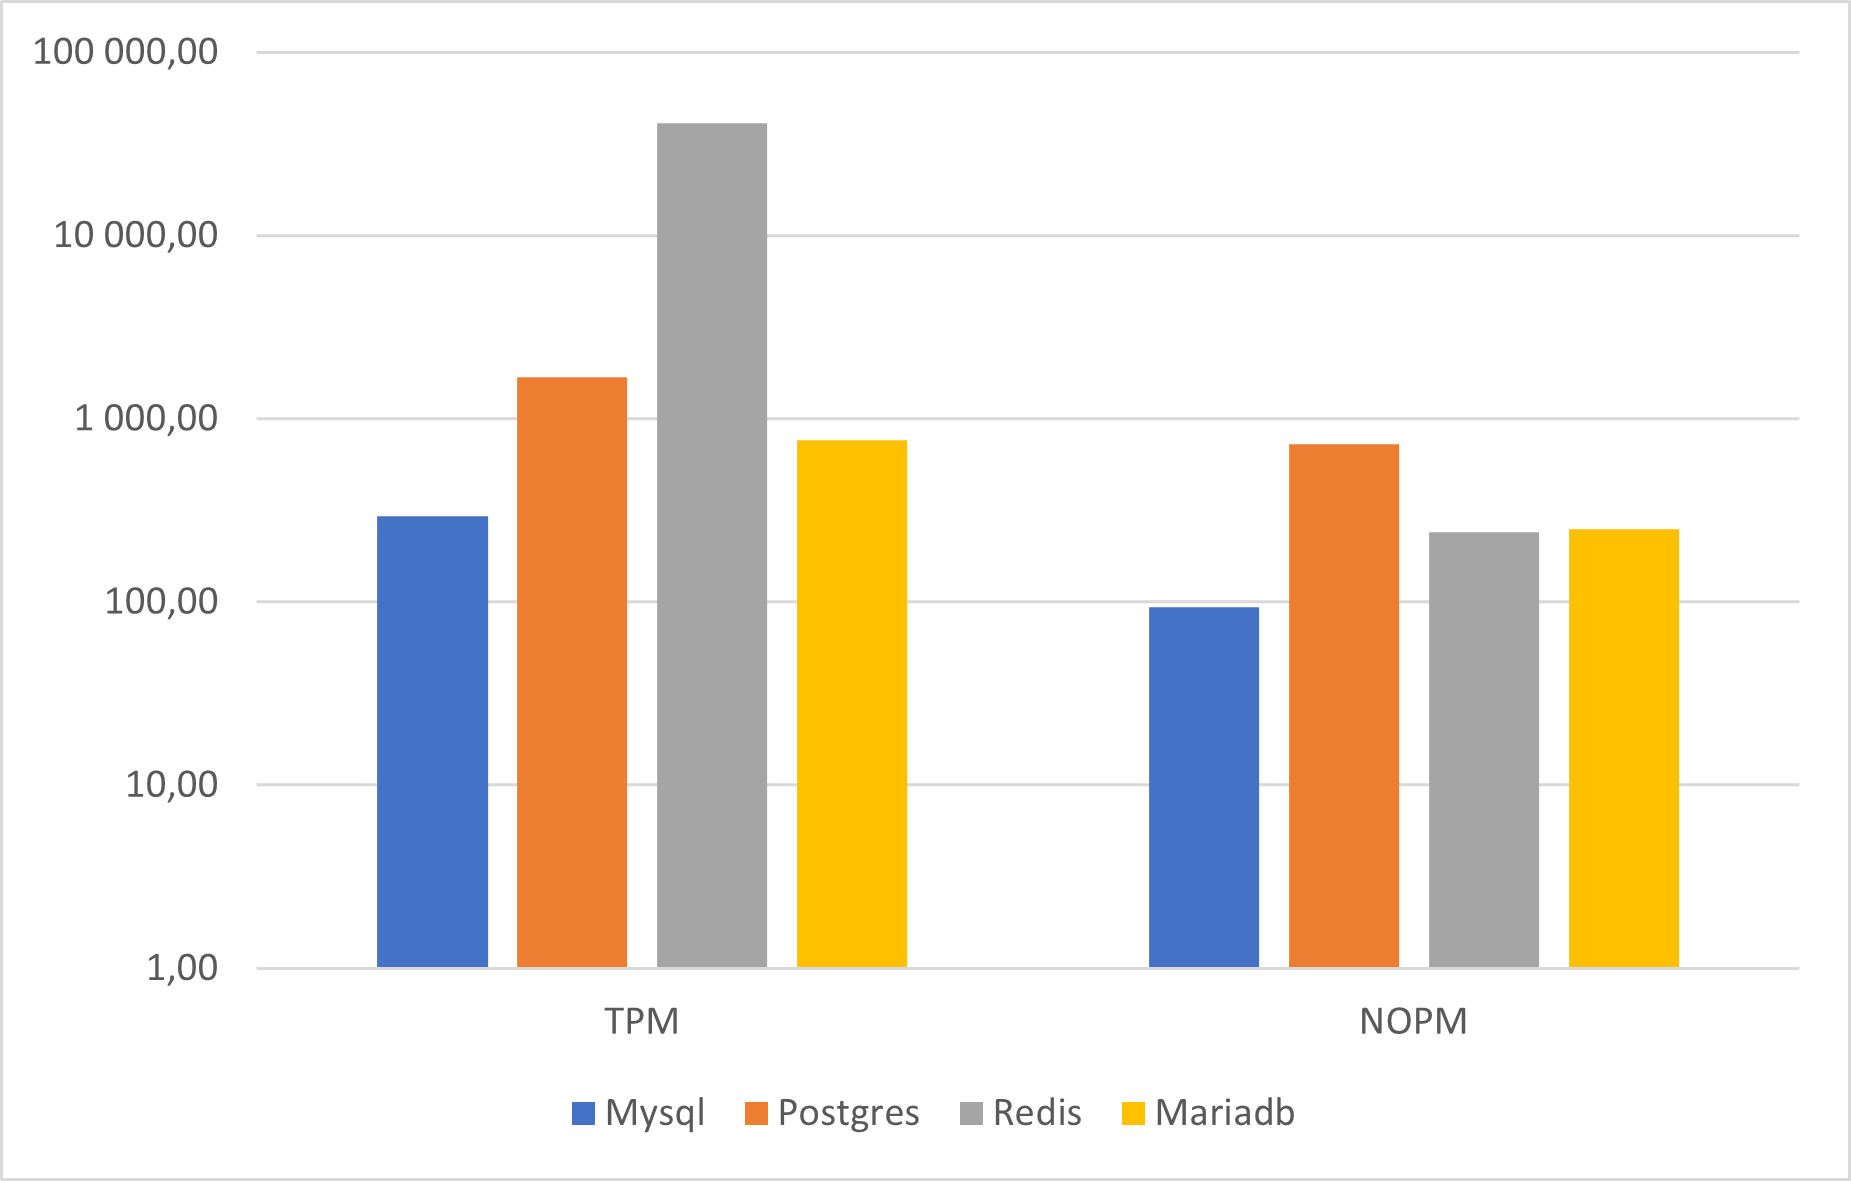
\includegraphics[width=0.6\columnwidth]{results/median/hammerdb.png}
\label{fig:medianhammerdb}
\end{figure*}


\begin{figure*}[h!]
\centering
\caption{Median of Energy consumption per Transitions per minute.}
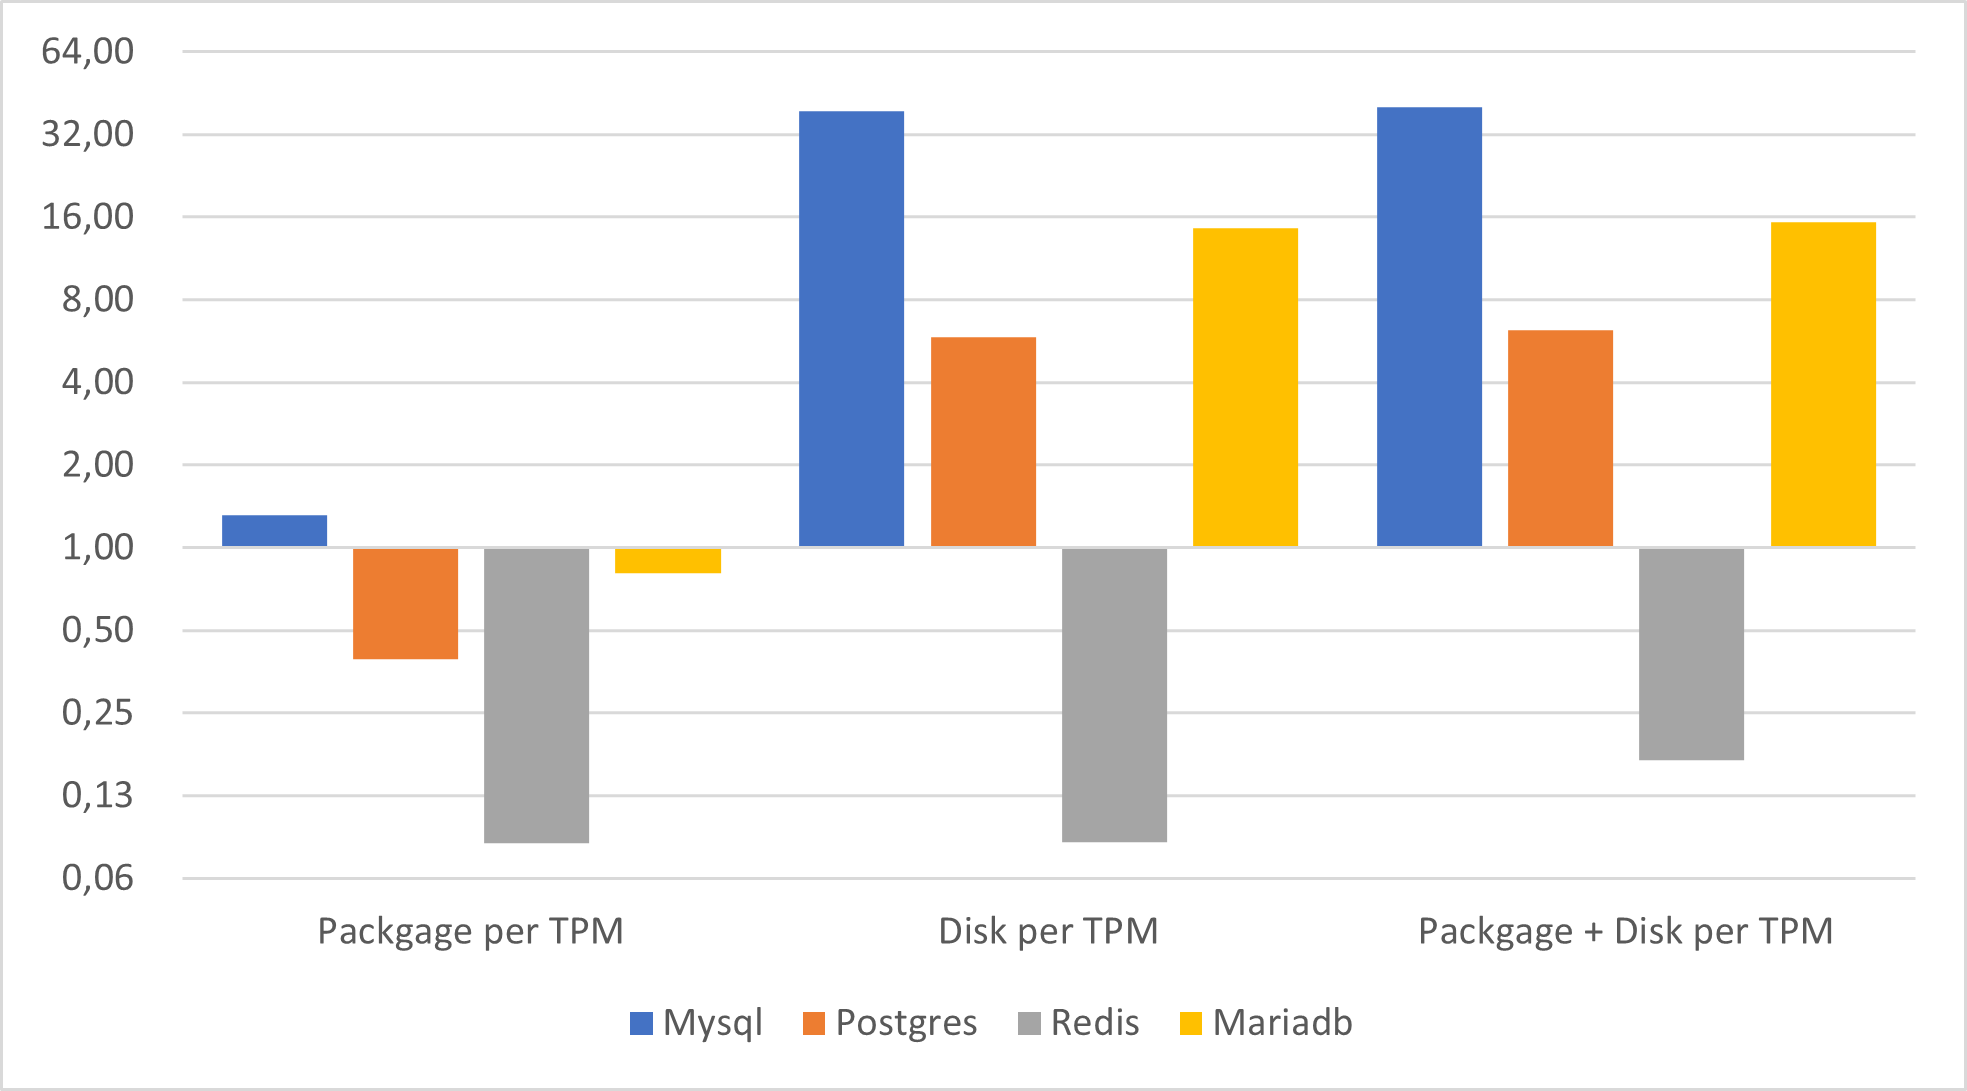
\includegraphics[width=0.6\columnwidth]{results/median/energy-tpm.png}
\label{fig:medianenergyhammerdb}	
\end{figure*}   

 \begin{figure*}[h!]
\centering
\caption{Median of Energy consumption per New orders per minute.}
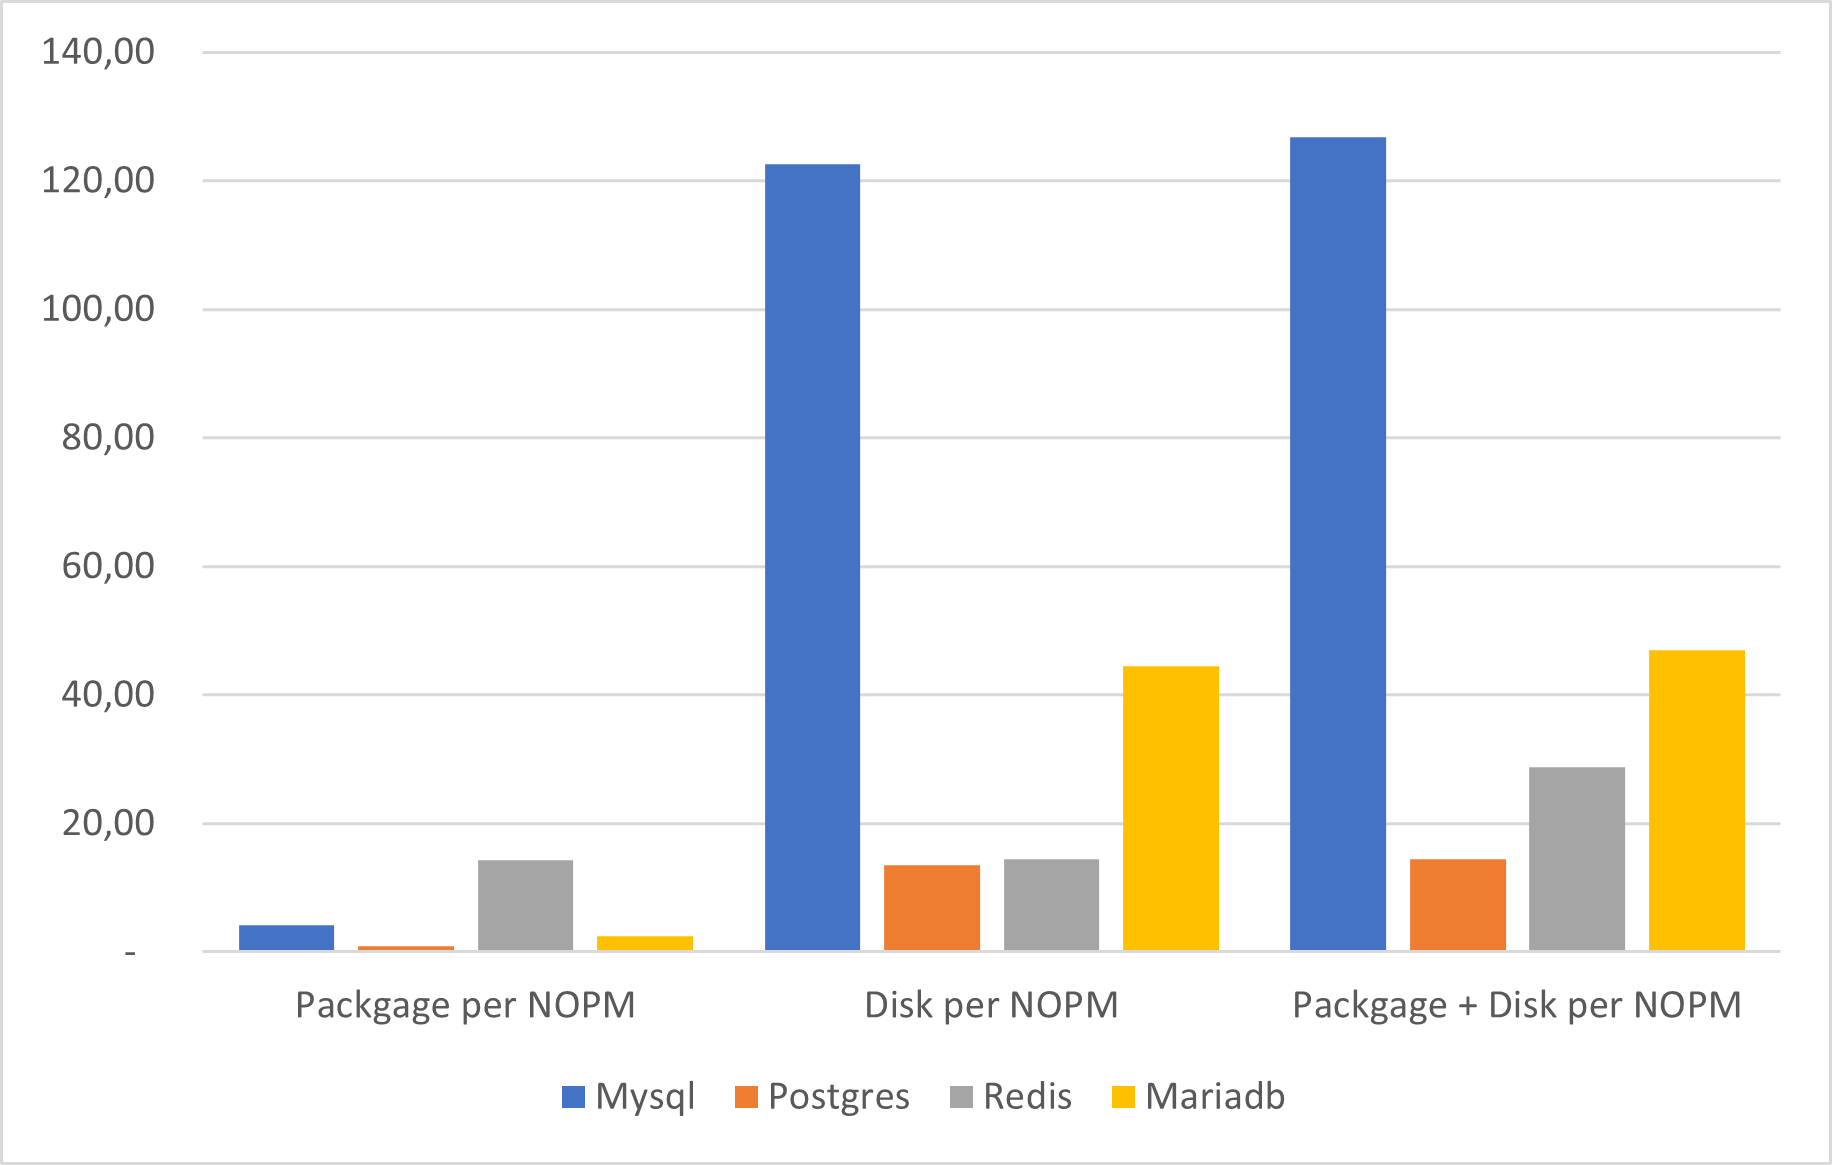
\includegraphics[width=0.6\columnwidth]{results/median/energy-nopm.png}
\label{fig:mediannopmenergy}	
\end{figure*}   
 %% Box plots
\begin{figure*}[h!]
\centering
\caption{Distribution of energy consumed.}
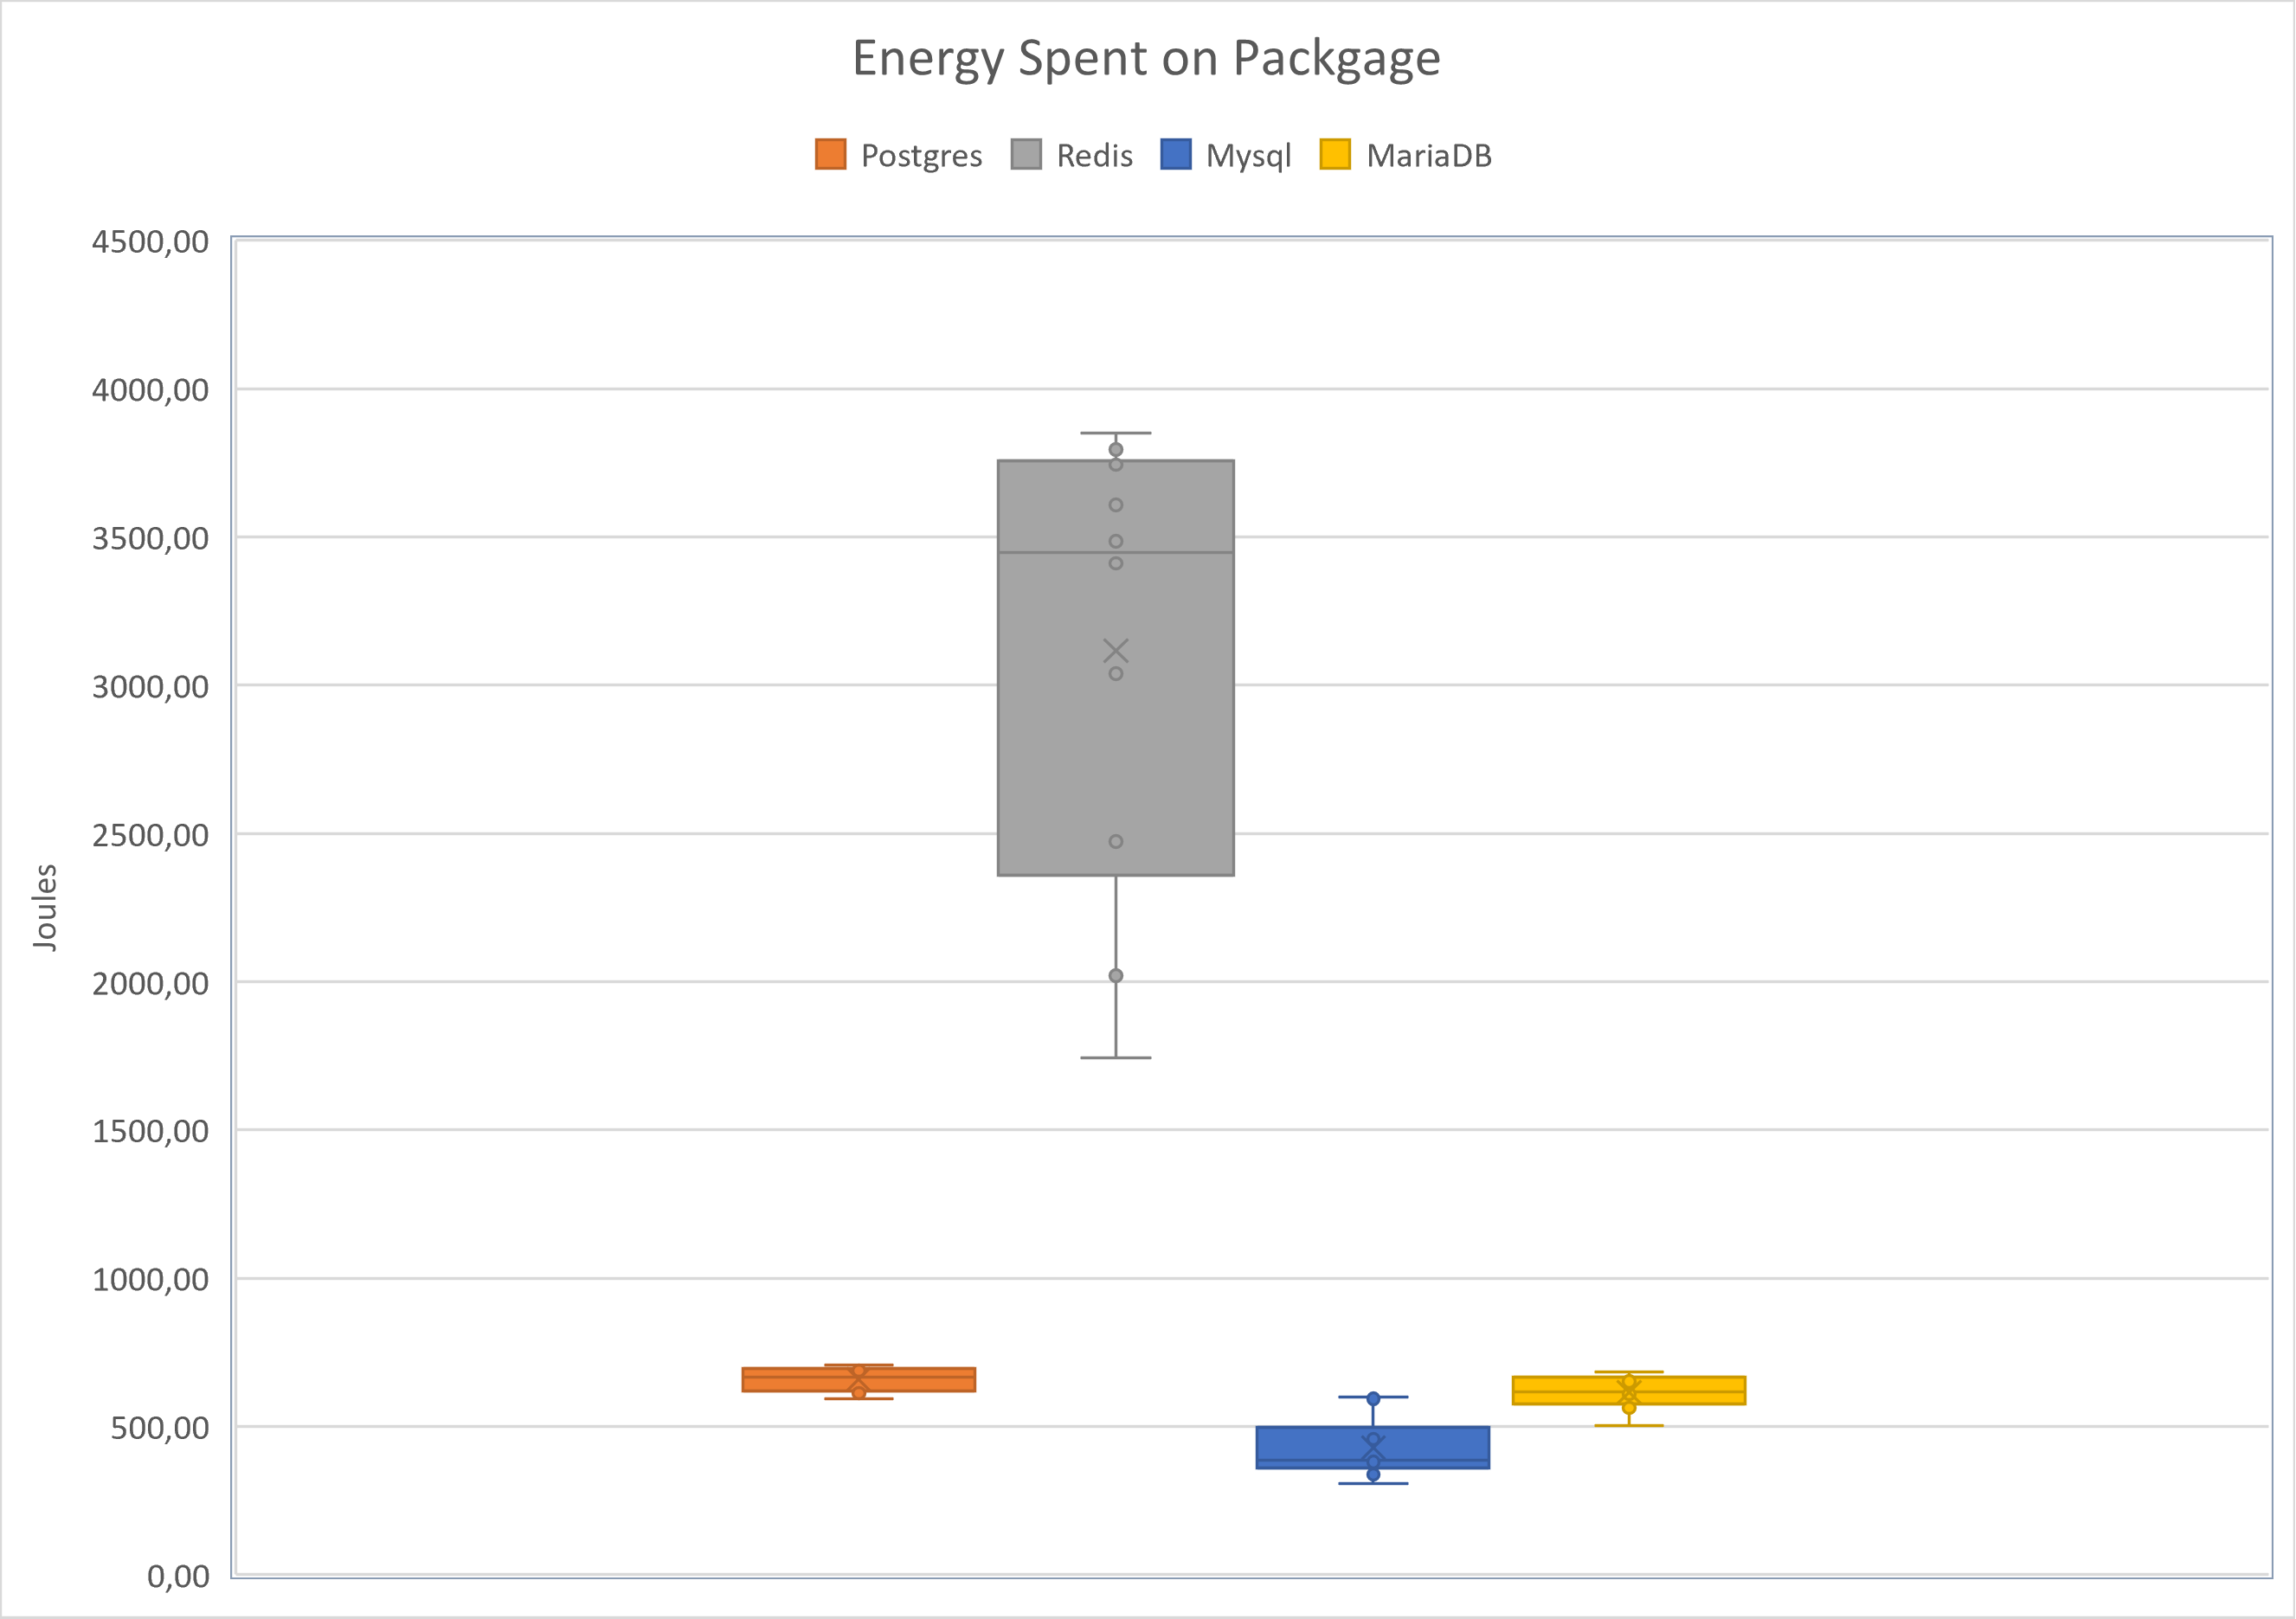
\includegraphics[width=0.5\columnwidth]{results/boxplot/Packgage.png}
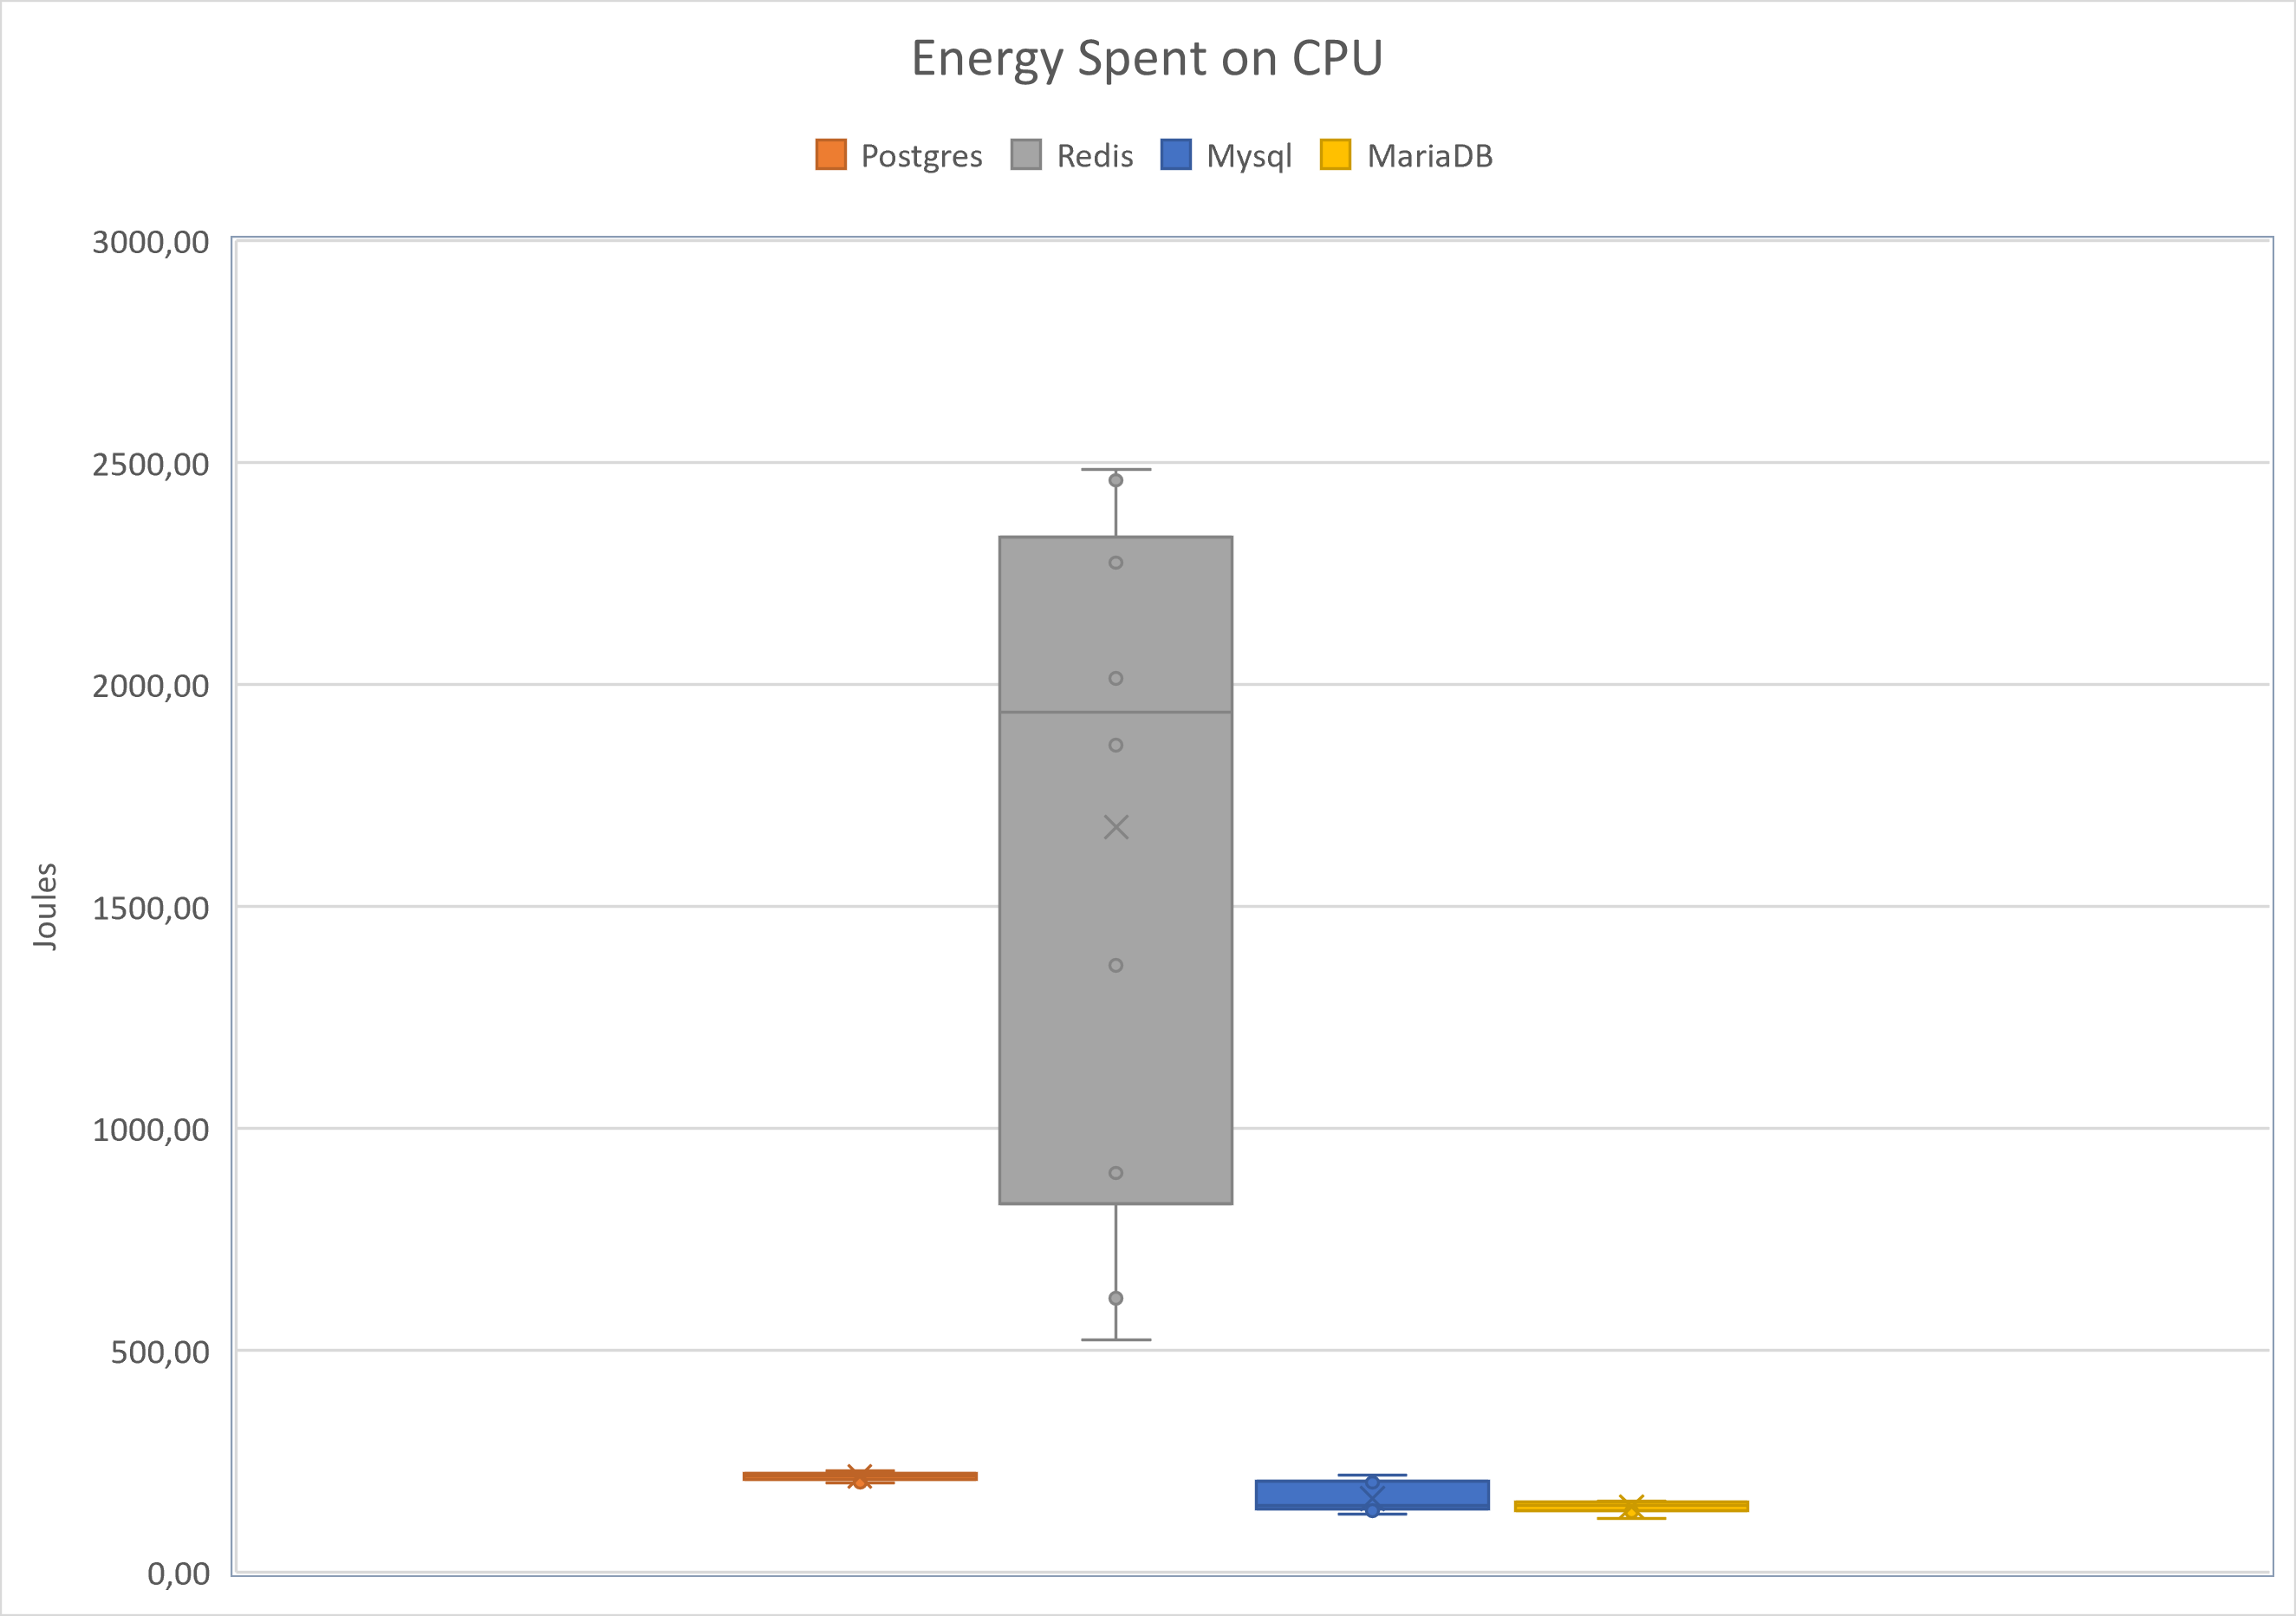
\includegraphics[width=0.5\columnwidth]{results/boxplot/CPU.png}
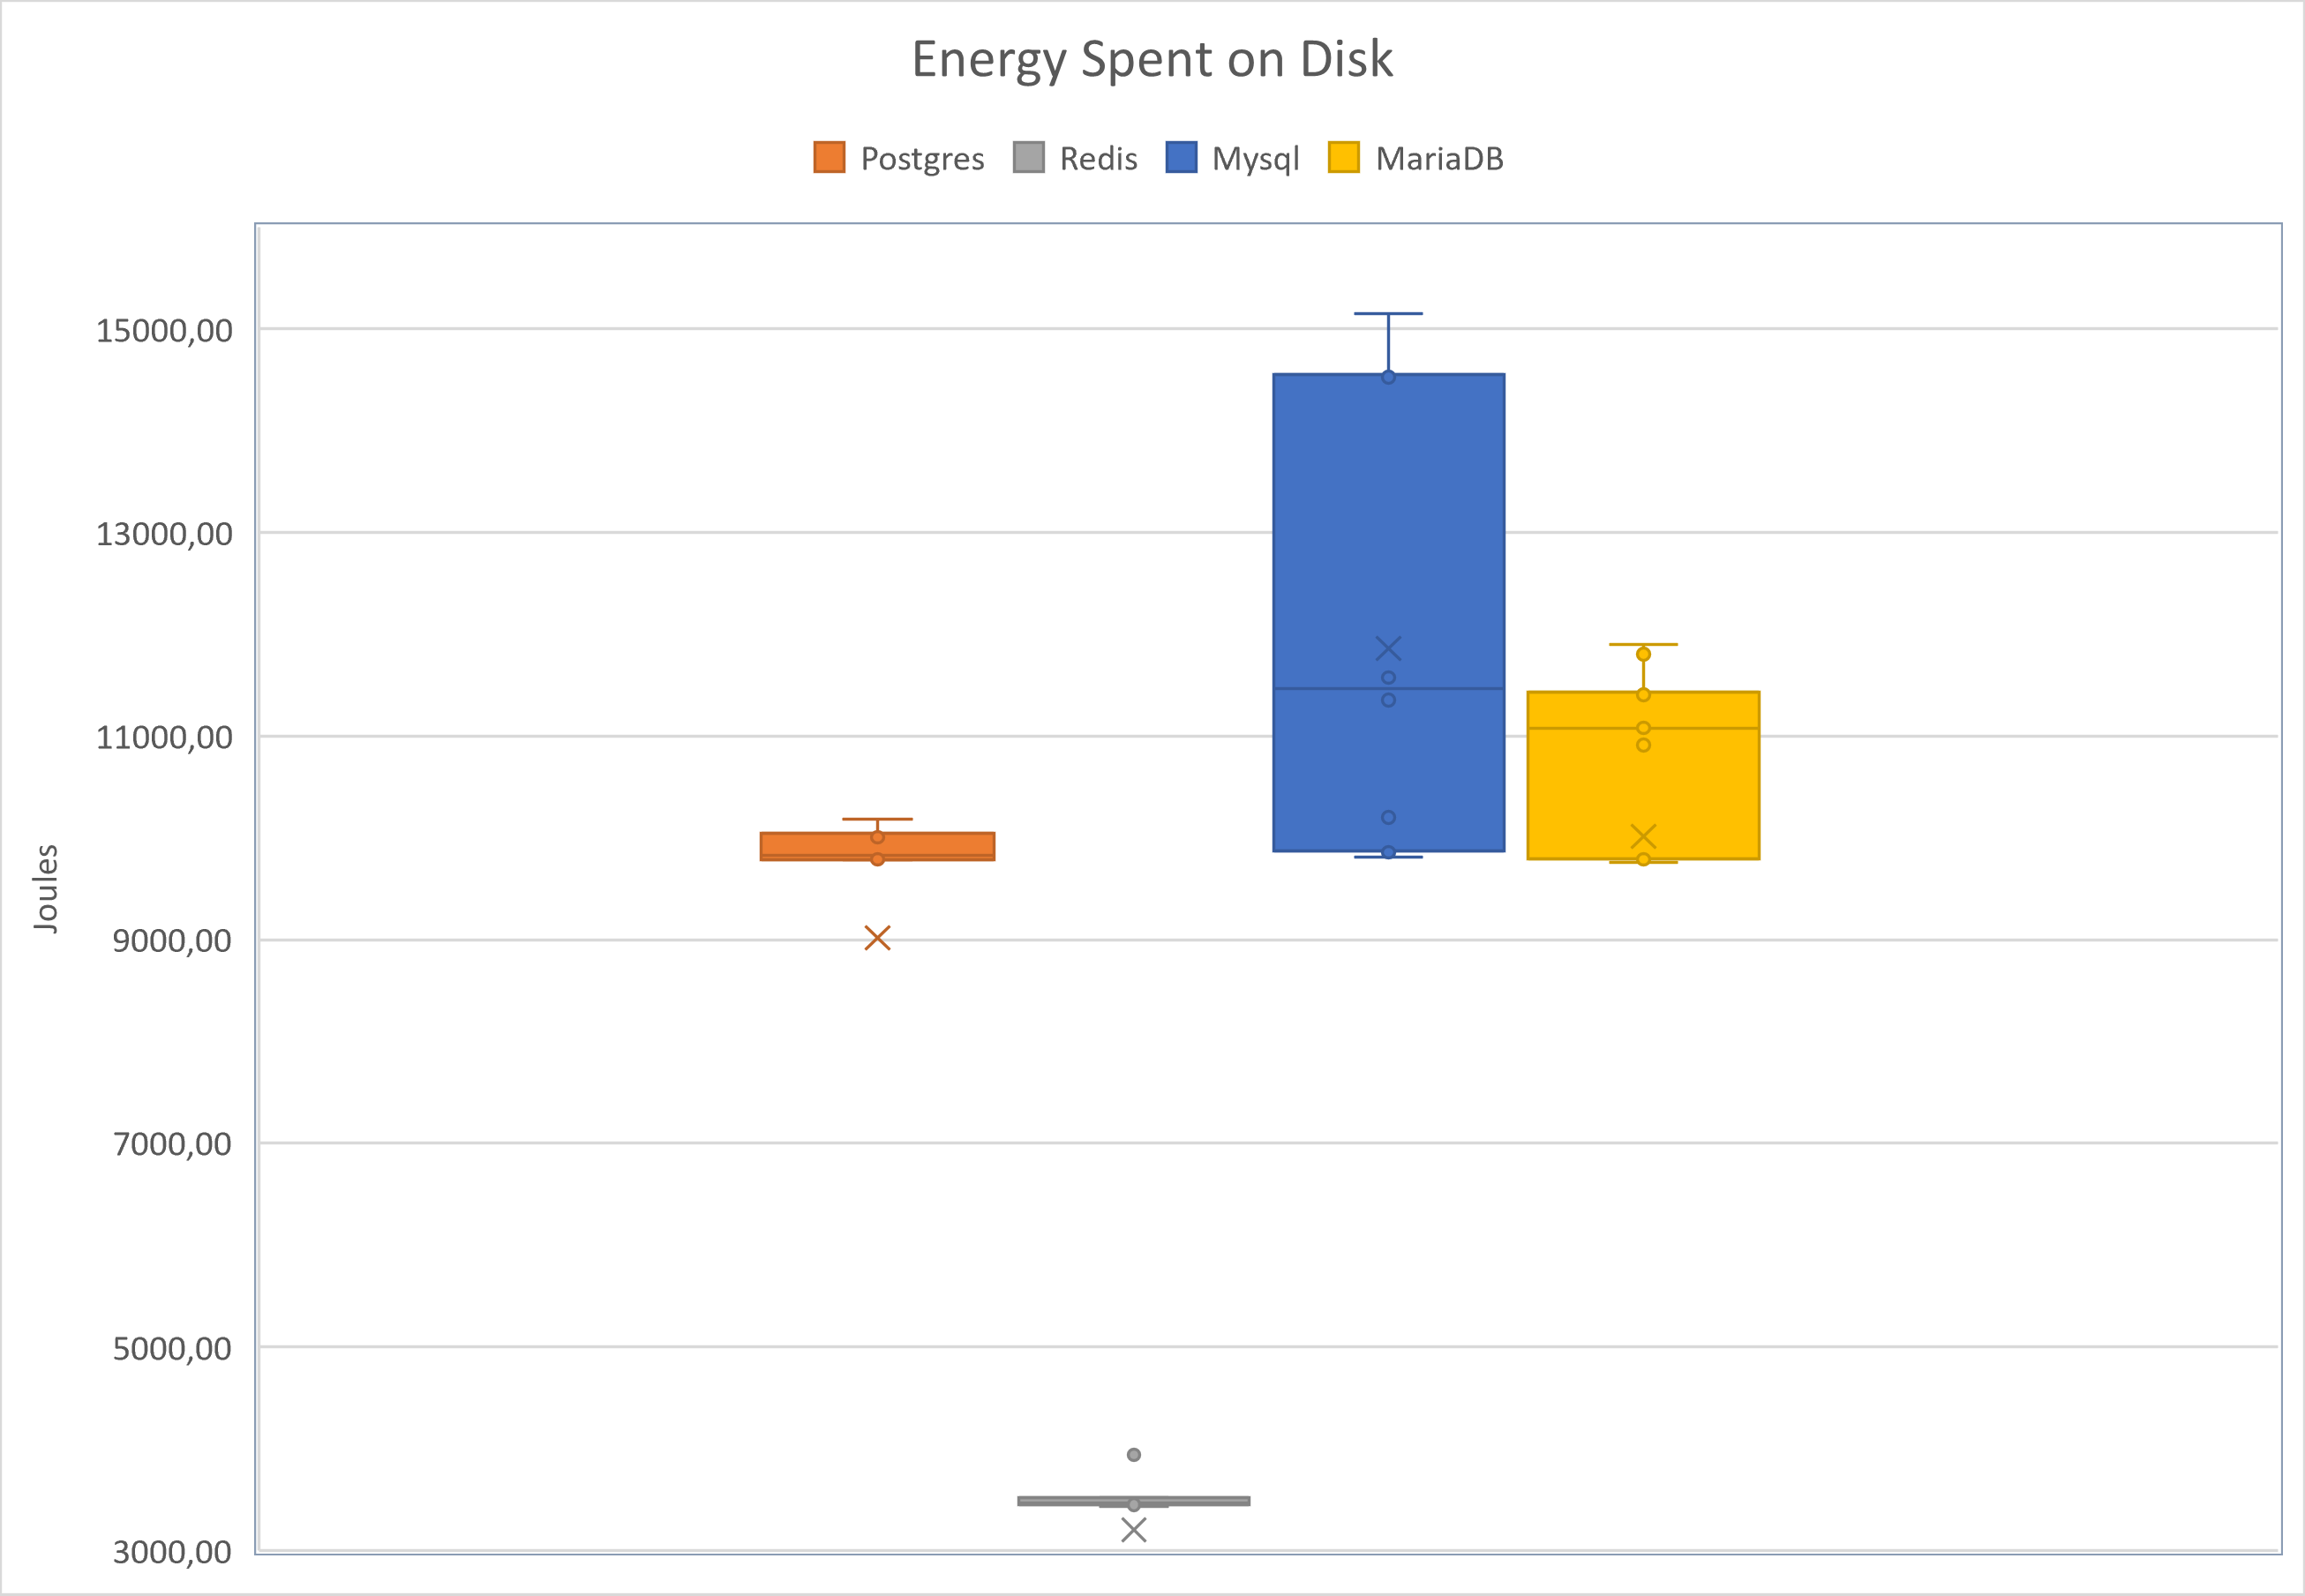
\includegraphics[width=0.5\columnwidth]{results/boxplot/Disk.png}
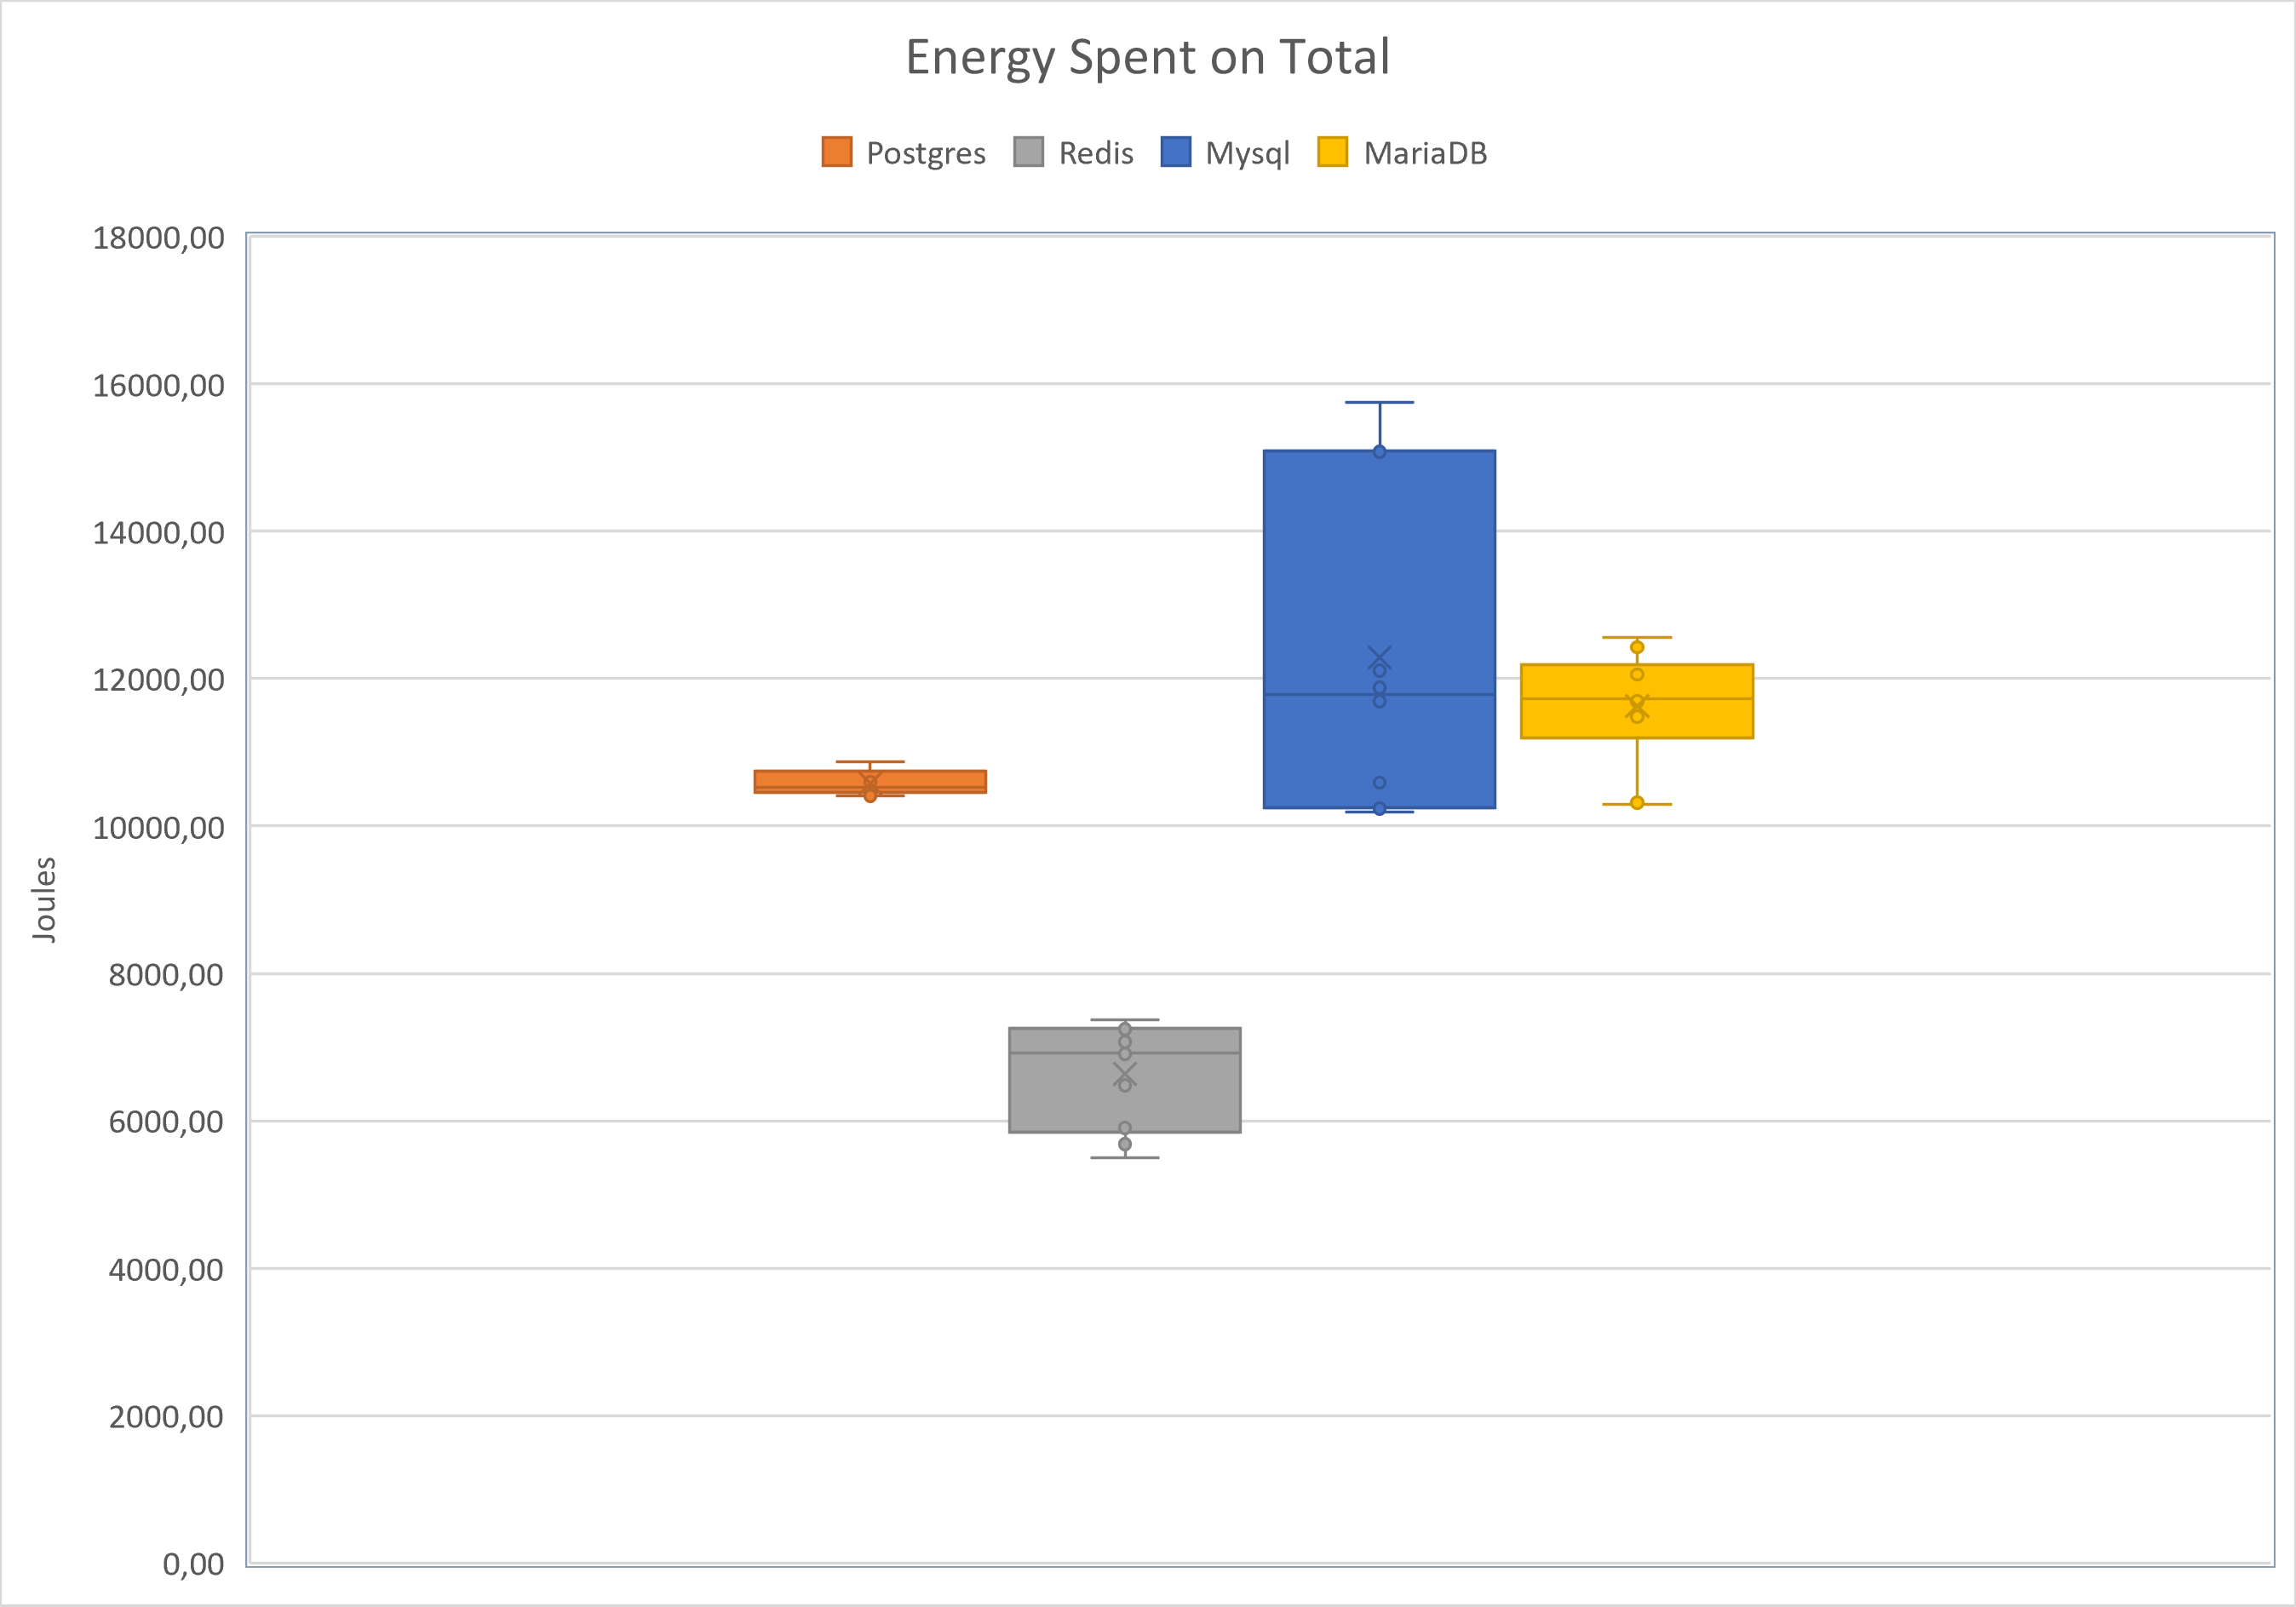
\includegraphics[width=0.5\columnwidth]{results/boxplot/Total.png}
\label{fig:bocplotyenergy}	
\end{figure*}
\begin{figure*}[h!]
\centering
\caption{Distribution of performance on HammerDB.}
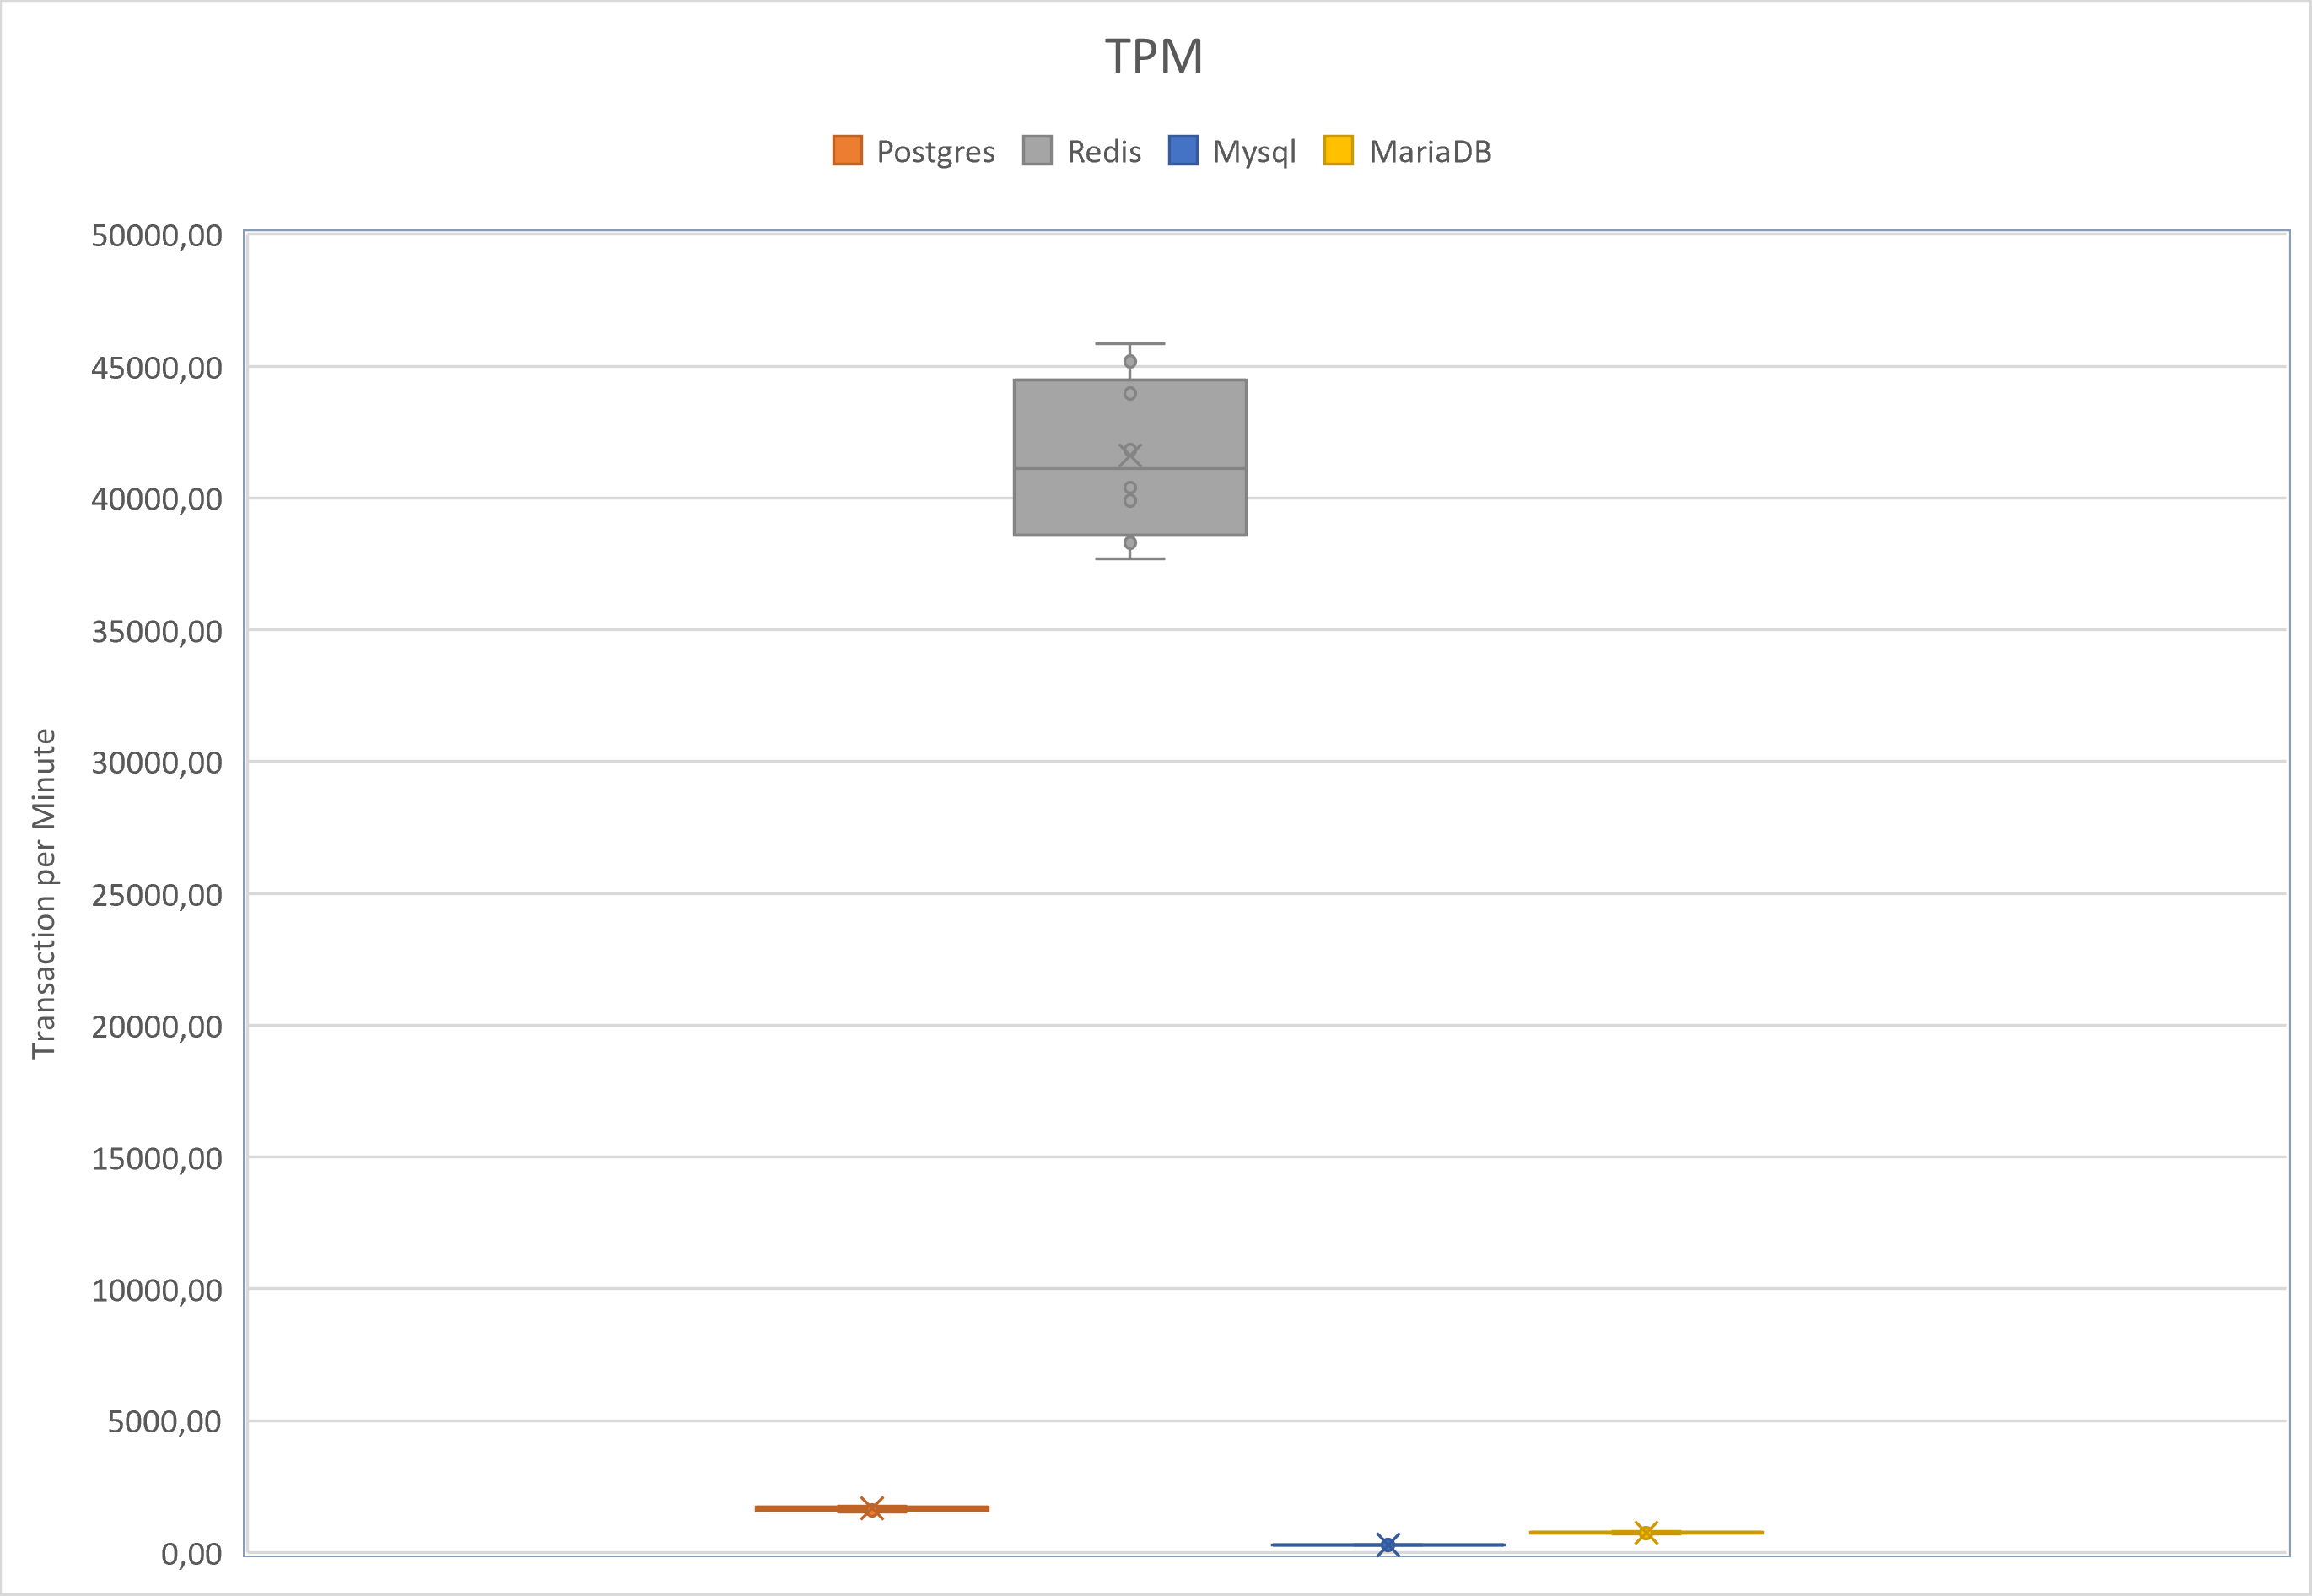
\includegraphics[width=0.6\columnwidth]{results/boxplot/TPM.png}
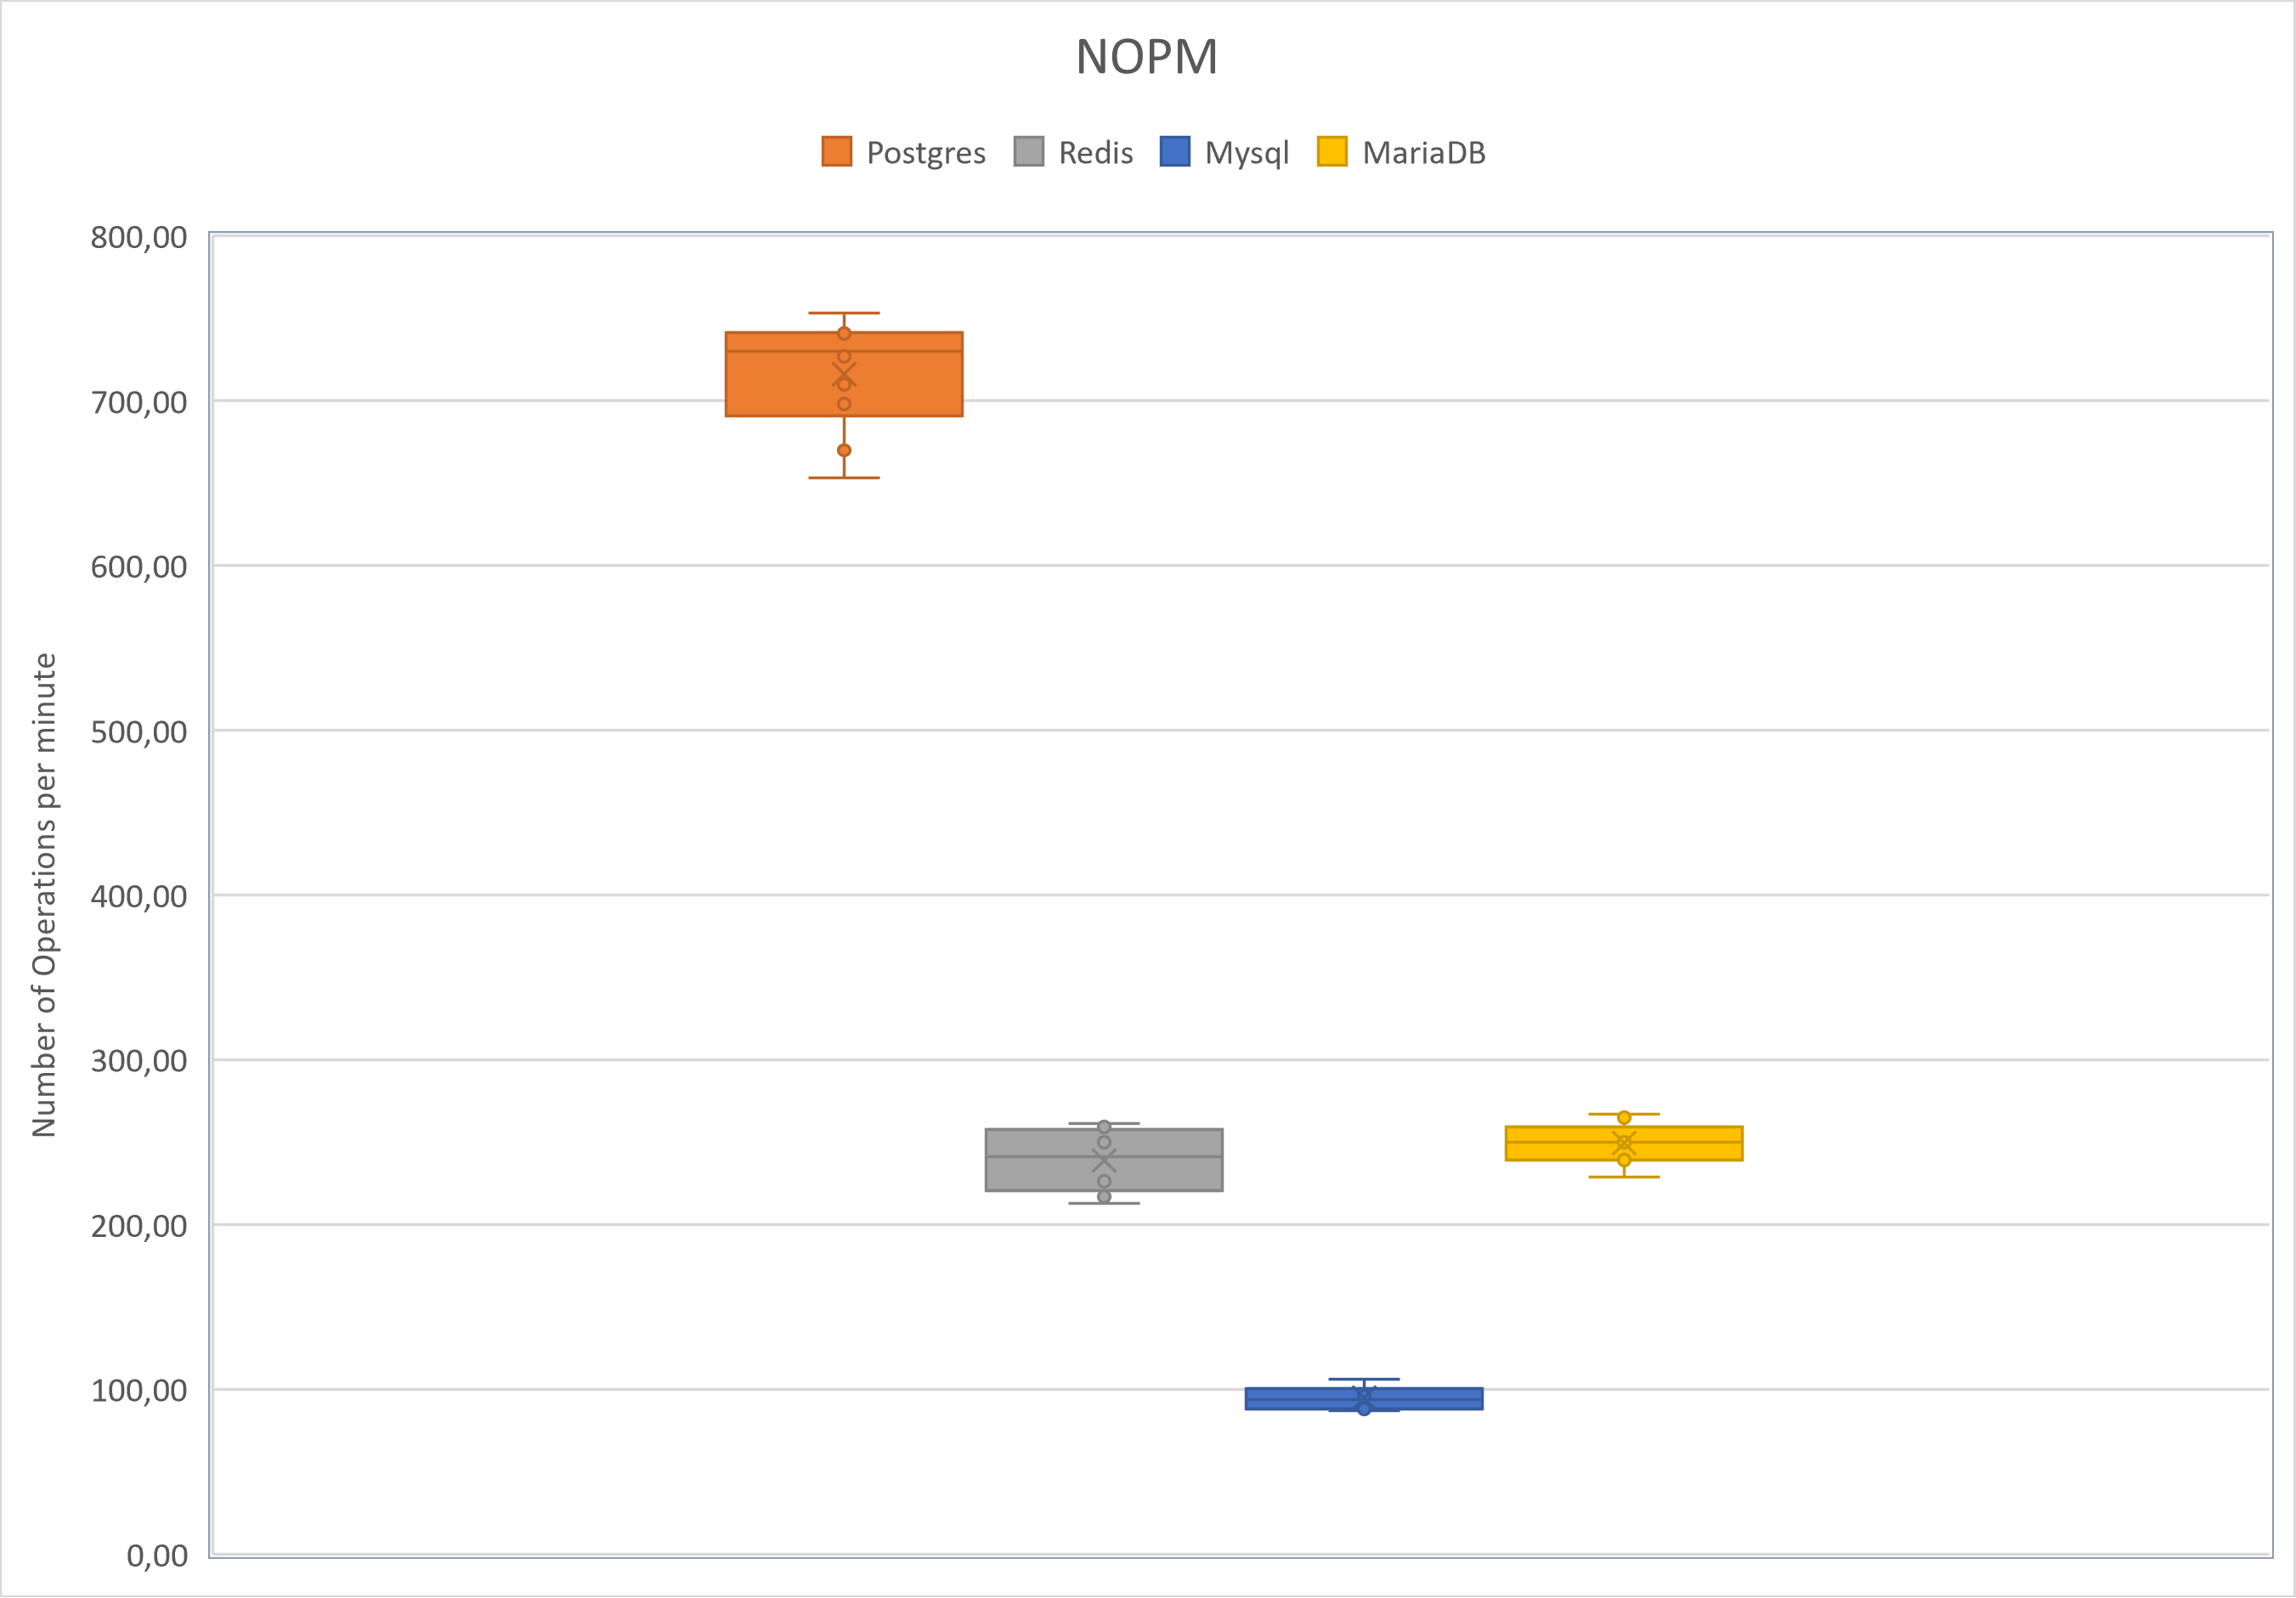
\includegraphics[width=0.6\columnwidth]{results/boxplot/NOPM.png}
\label{fig:bocplothammer}	
\end{figure*}

\begin{figure*}[h!]
\centering
\caption{Distribution of energy consumption per Transitions per minute.}
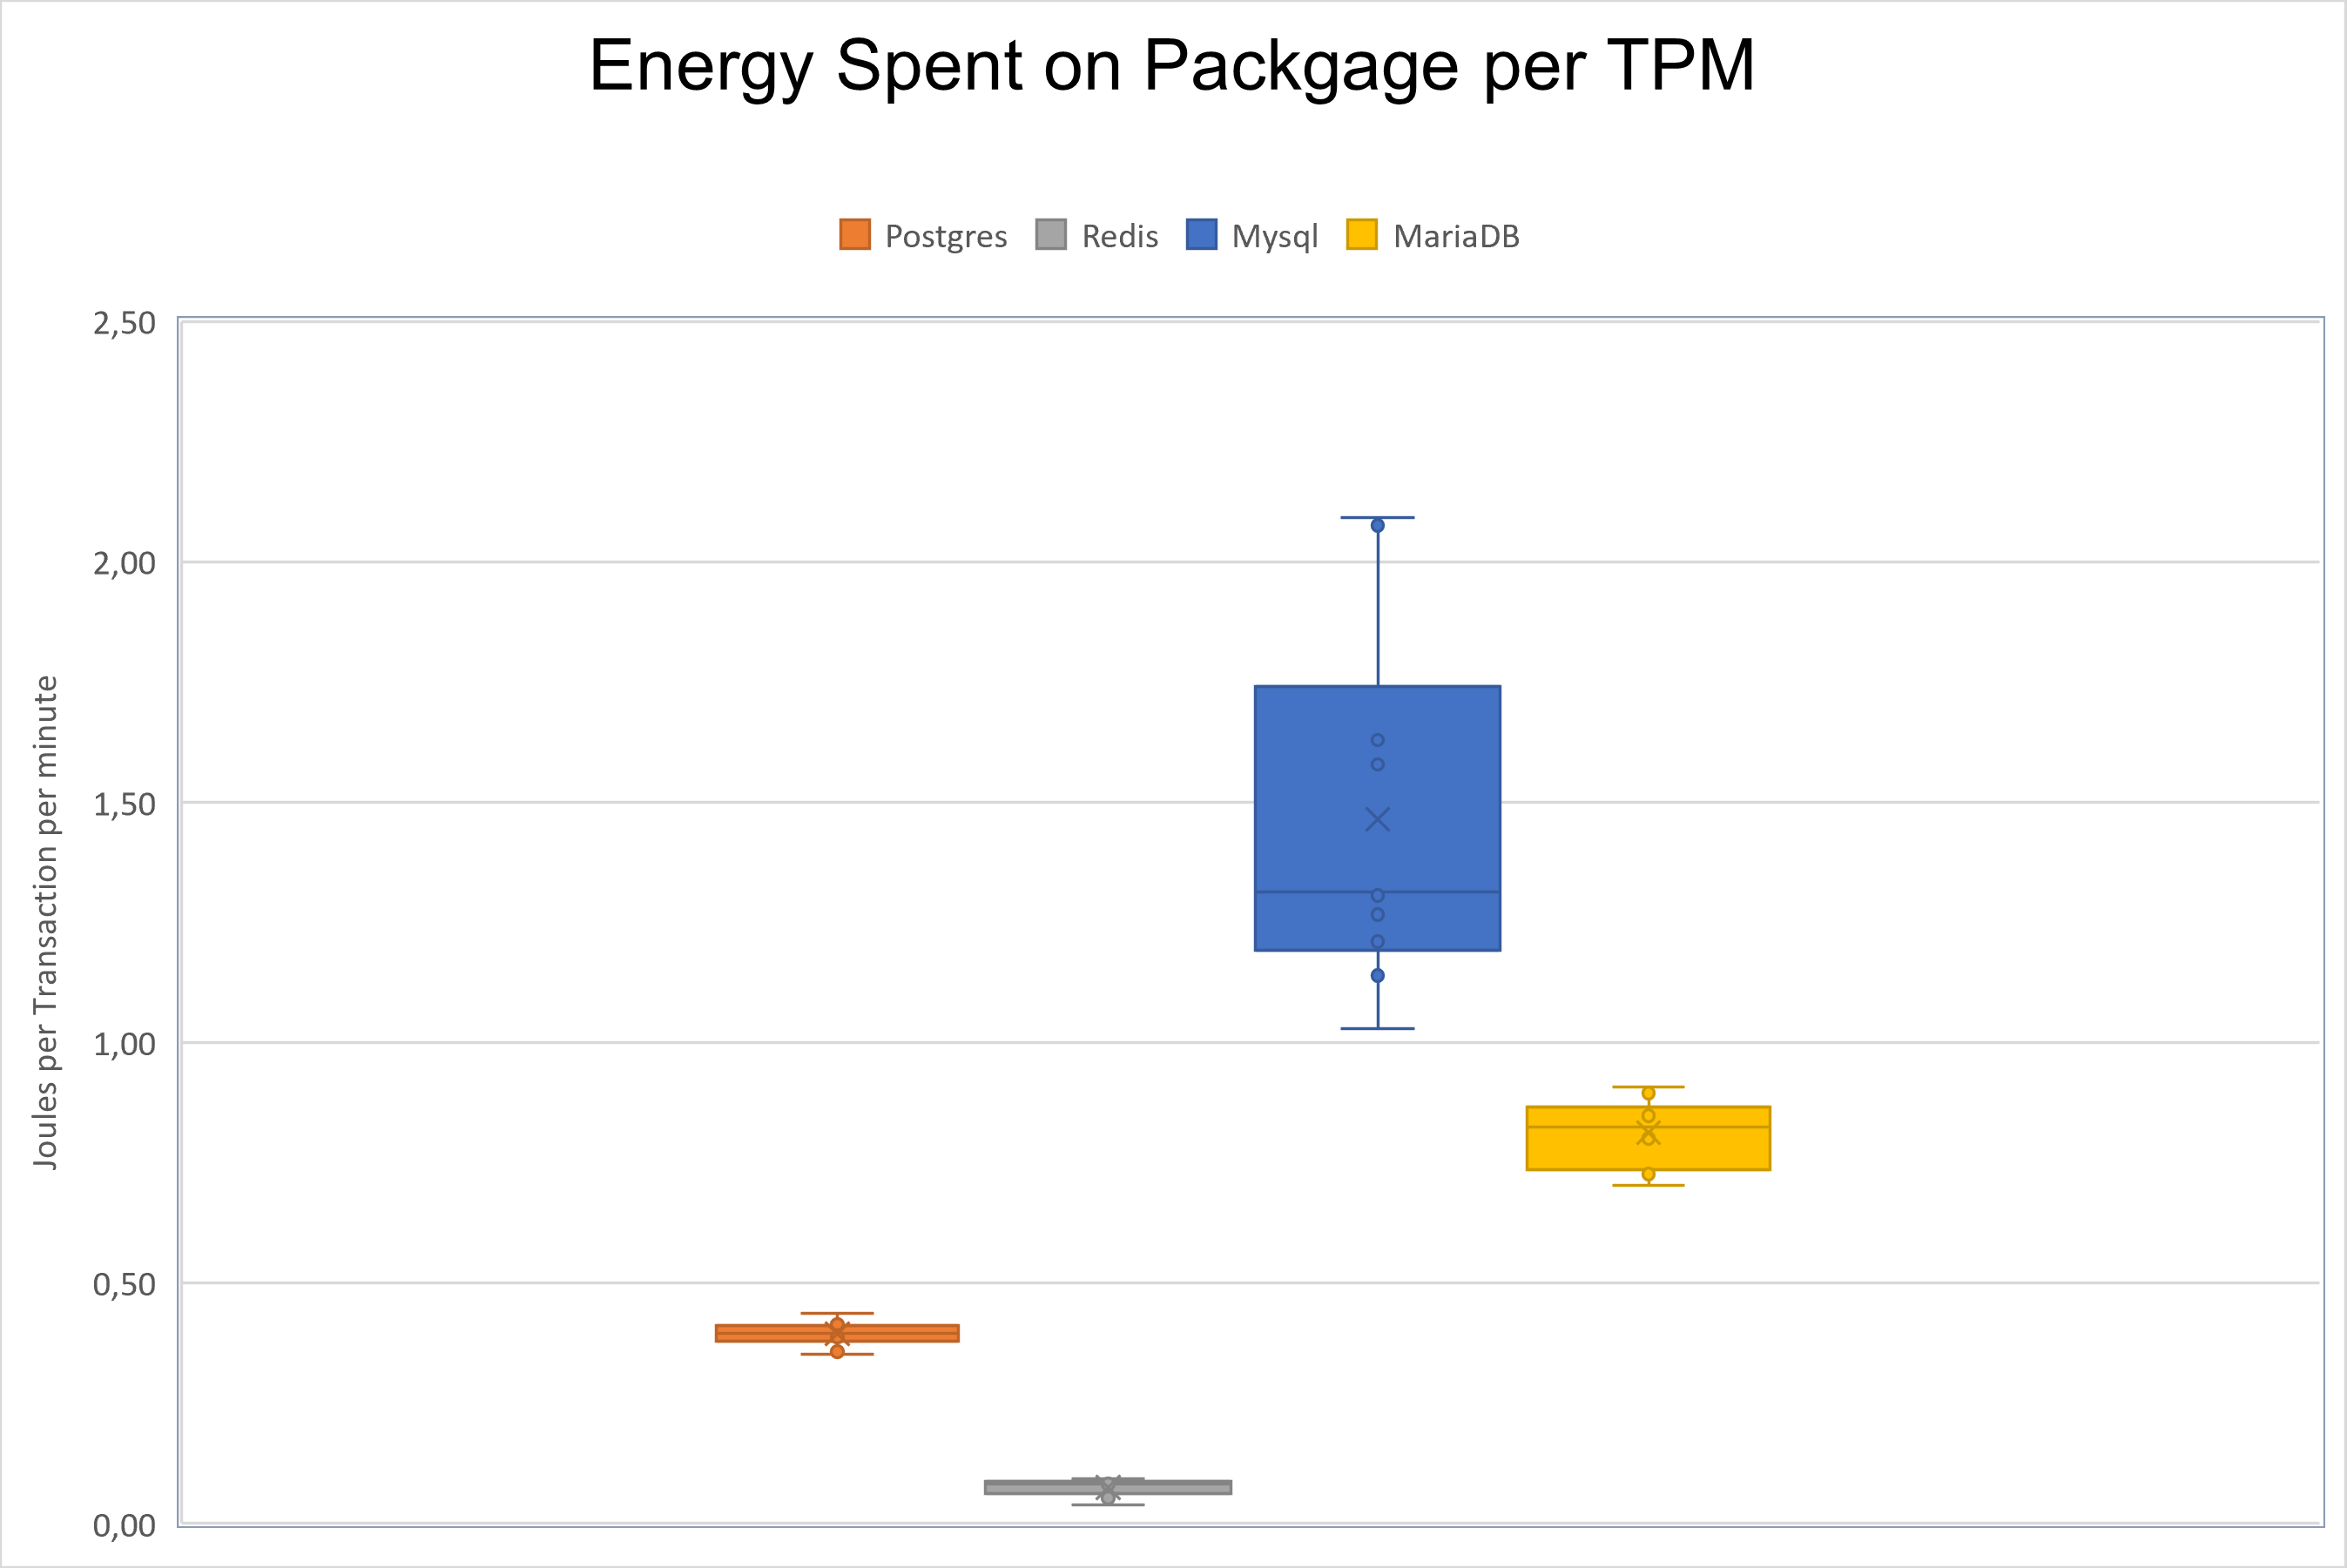
\includegraphics[width=0.6\columnwidth]{results/boxplot/Packgage-tpm.png}
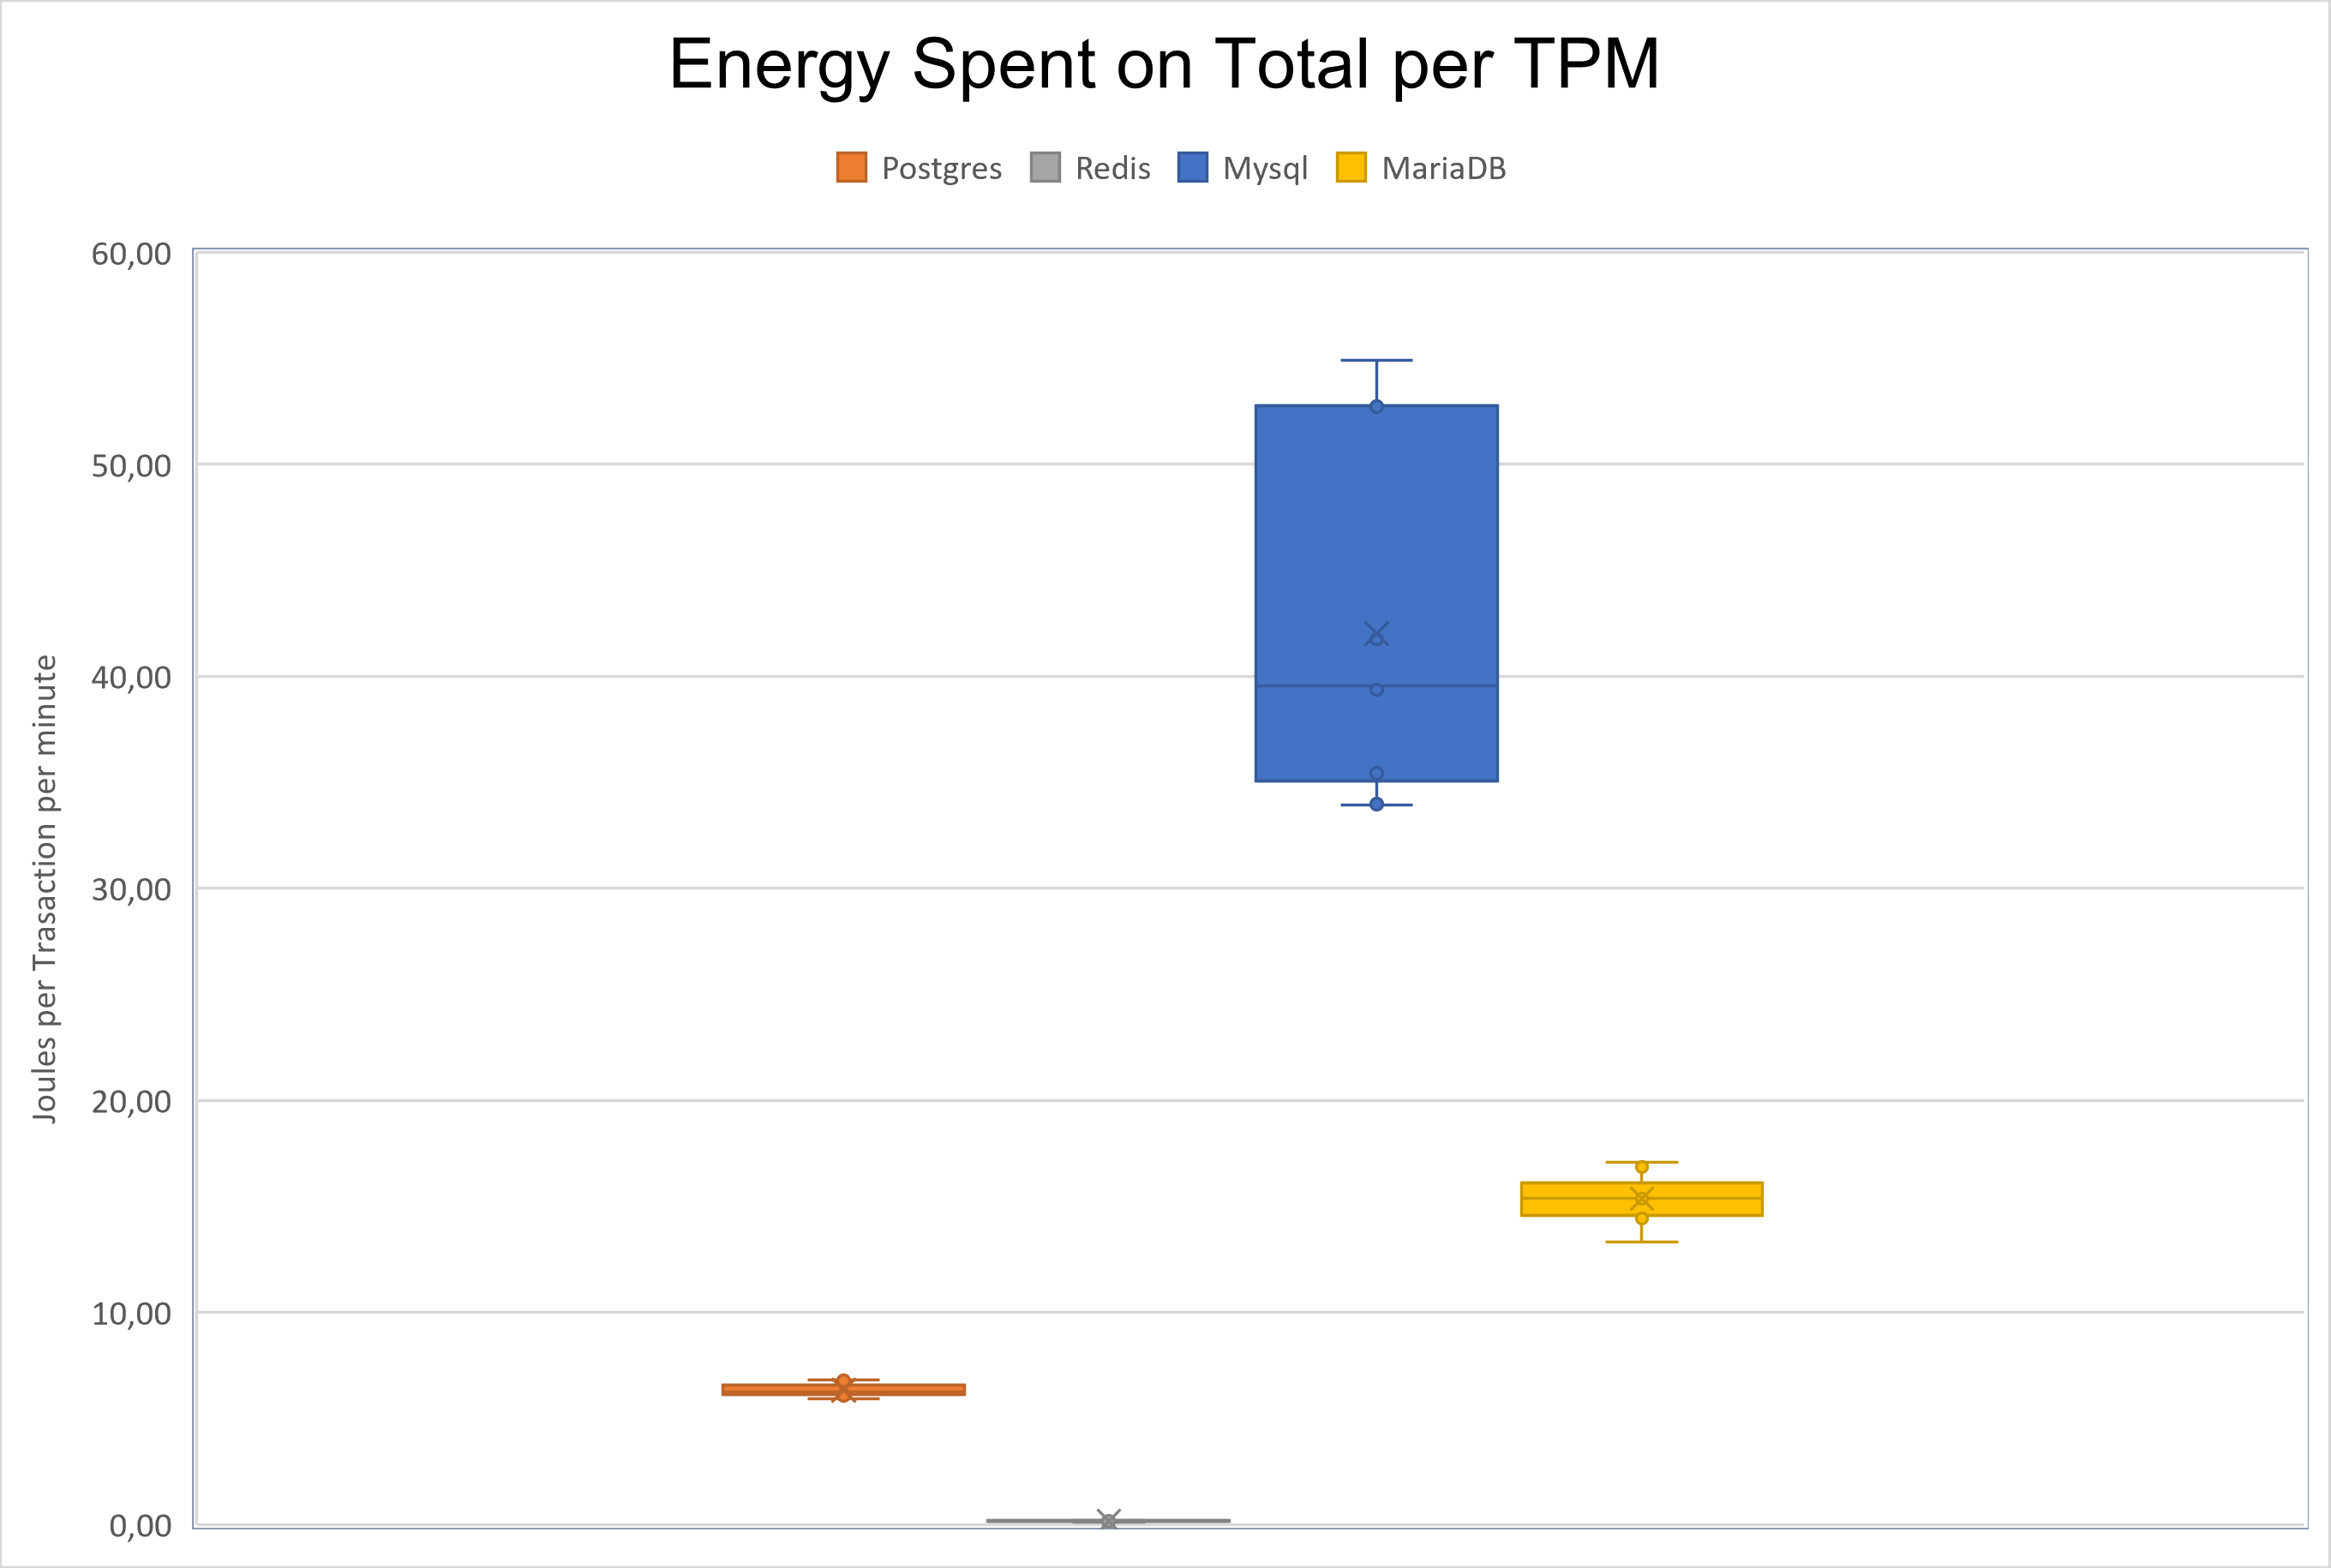
\includegraphics[width=0.6\columnwidth]{results/boxplot/total-tpm.png}
\includegraphics[width=0.6\columnwidth]{results/boxplot/Disk-tpm.png}
\label{fig:bocplottrans}	
\end{figure*}

\begin{figure*}[h!]
\centering
\caption{Distribution of energy consumption per New orders per minute.}
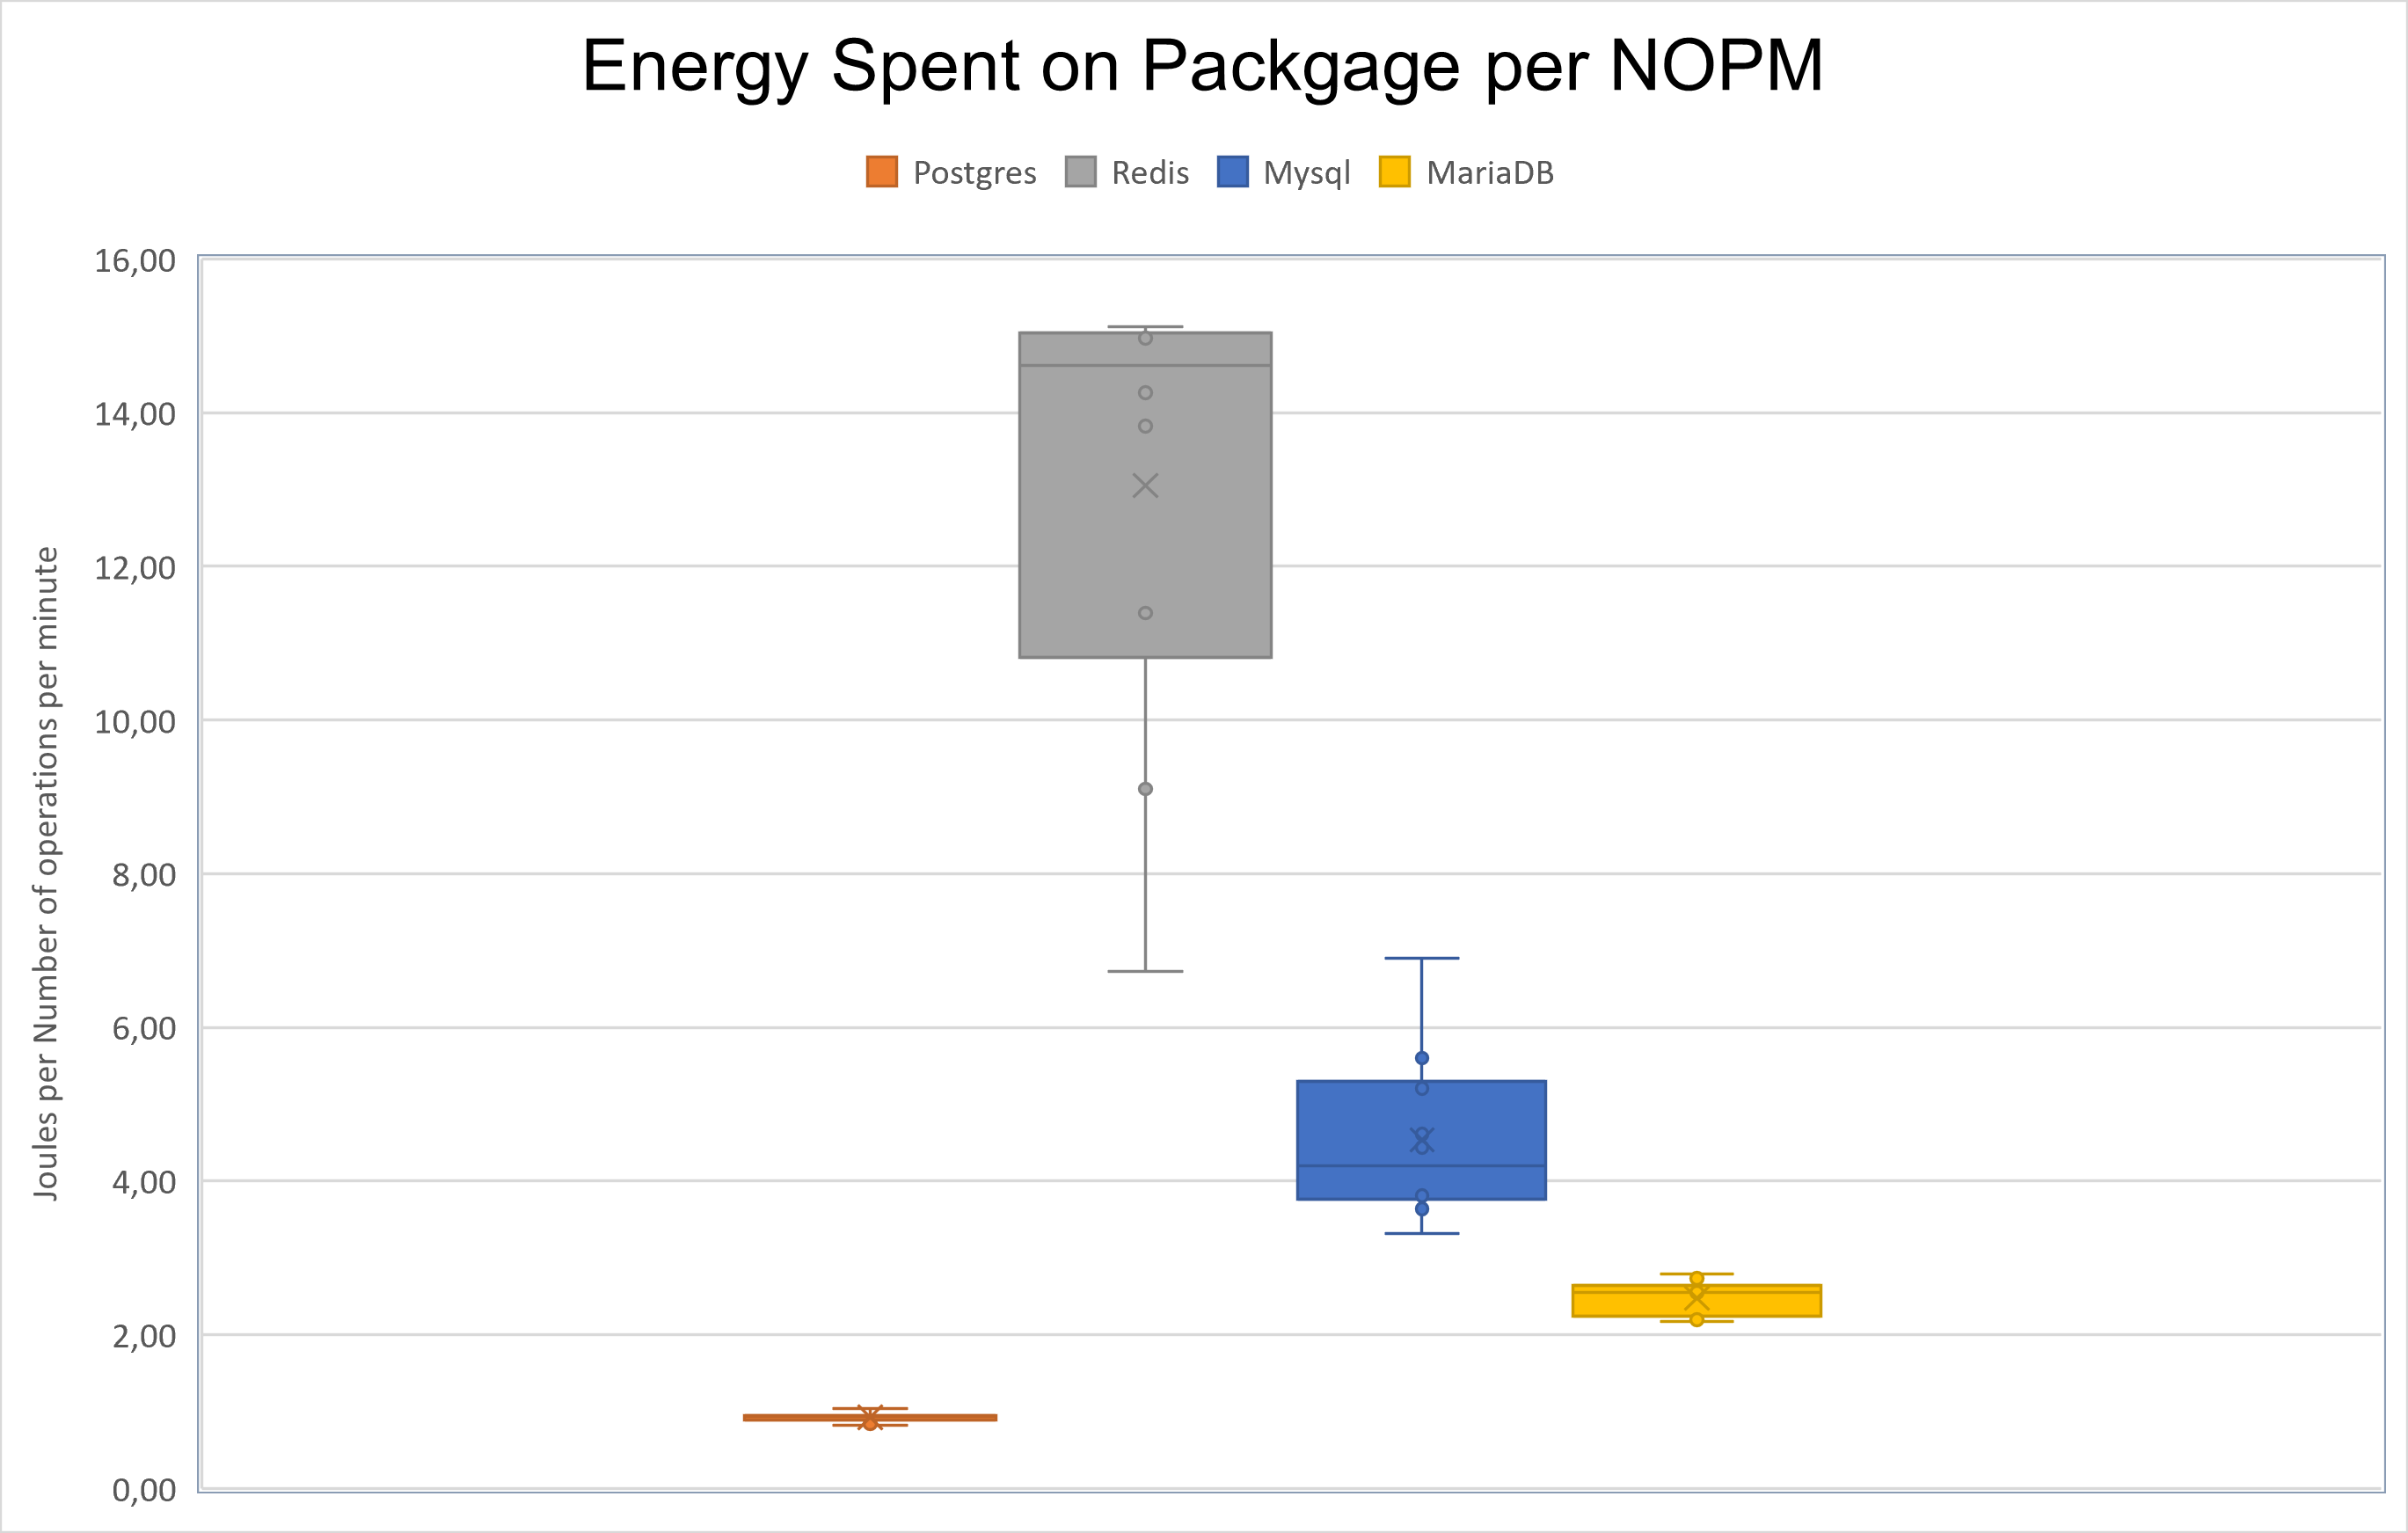
\includegraphics[width=0.6\columnwidth]{results/boxplot/Packgage-nopm.png}
\includegraphics[width=0.6\columnwidth]{results/boxplot/Disk-nopm.png}
\includegraphics[width=0.6\columnwidth]{results/boxplot/Total-nopm.png}
\label{fig:bocplotnumber}	
\end{figure*}


%% VUS
\begin{figure*}[h!]
\centering
\caption{Energy consumption with different number of users.}
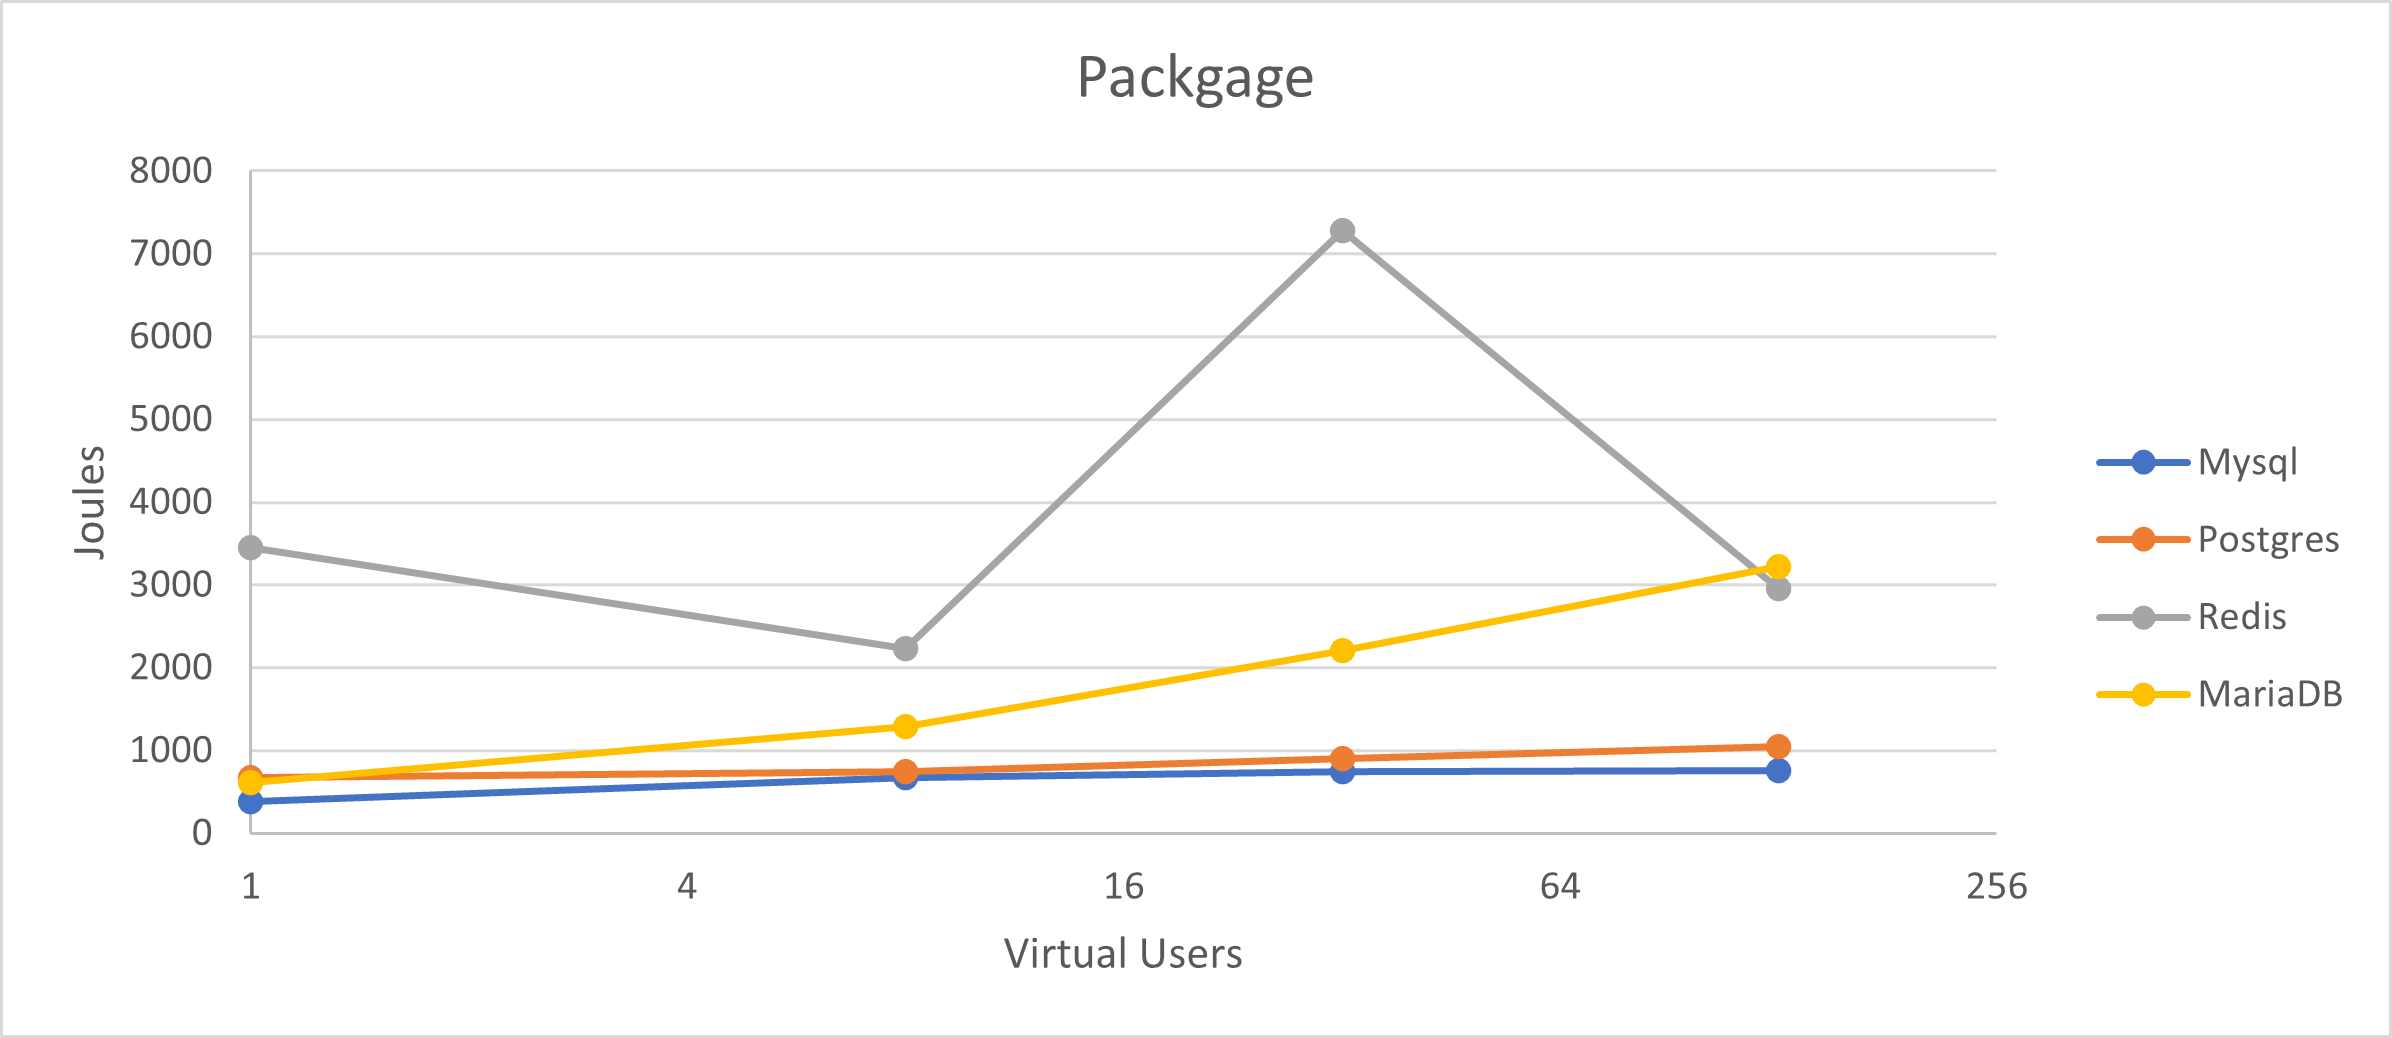
\includegraphics[width=0.76\columnwidth]{results/vu/Packgage.png}
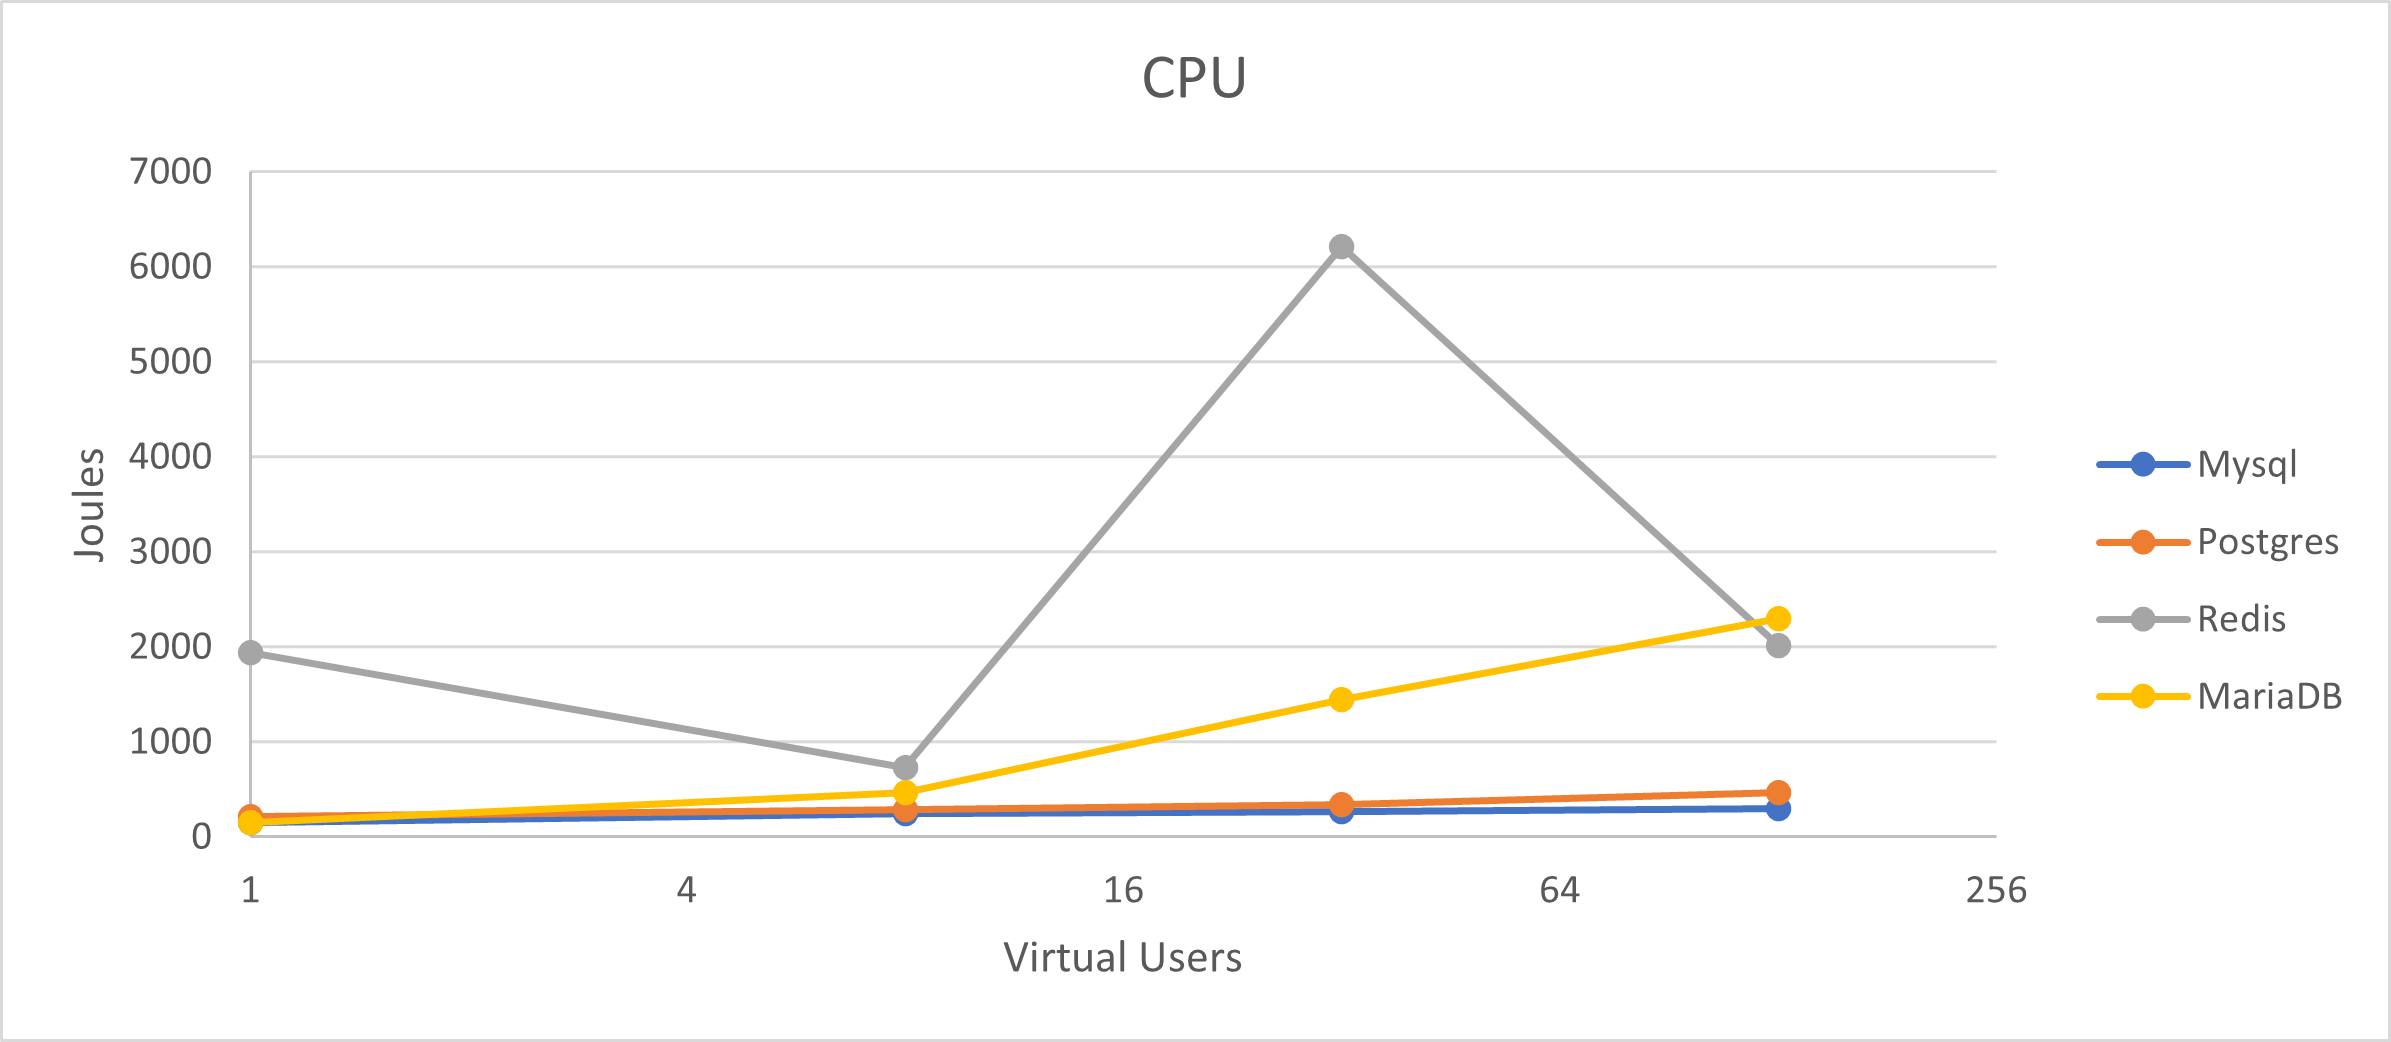
\includegraphics[width=0.76\columnwidth]{results/vu/CPU.png}
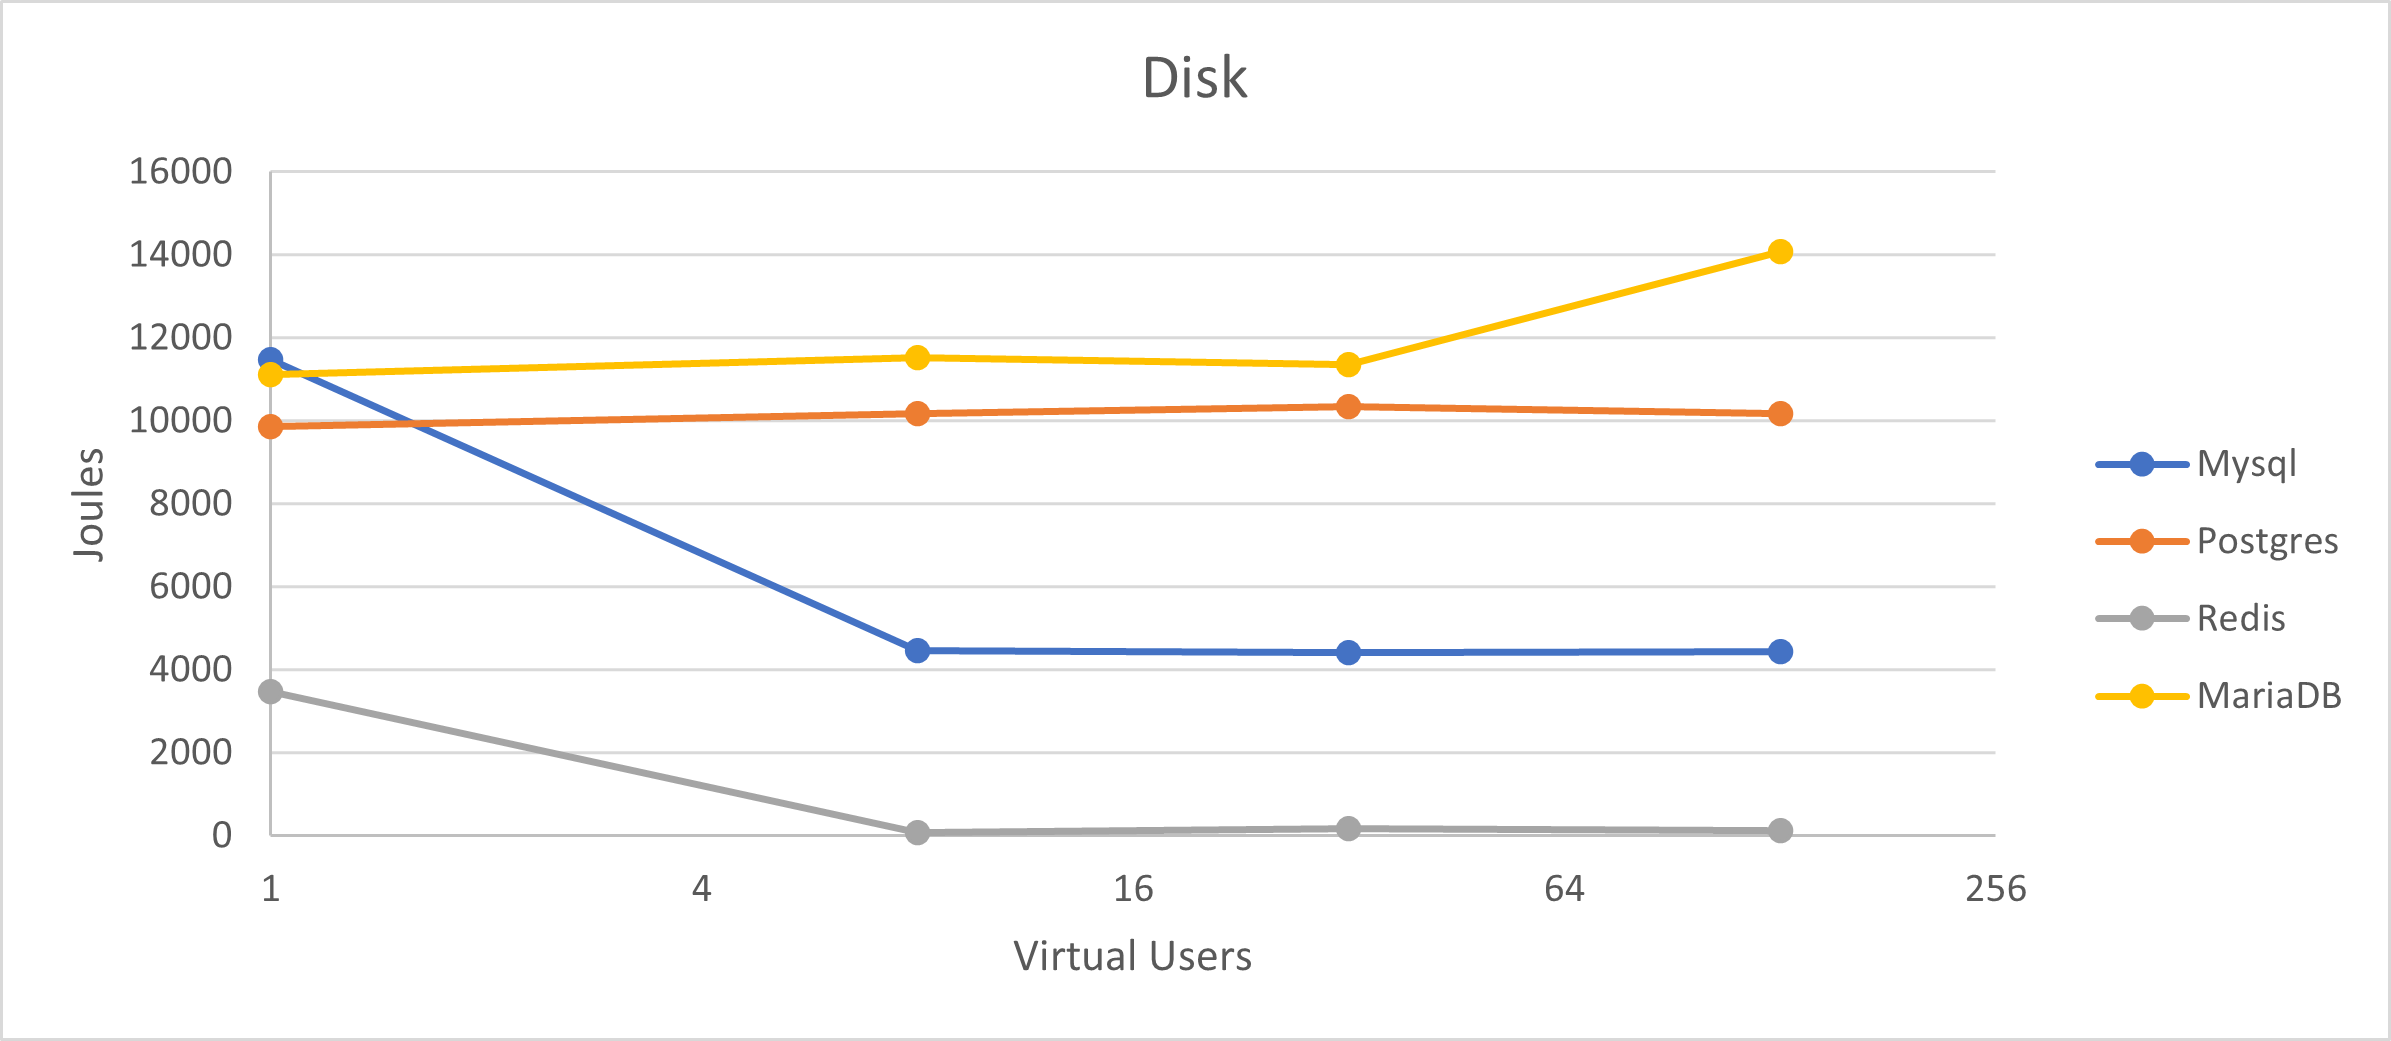
\includegraphics[width=0.76\columnwidth]{results/vu/Disk.png}
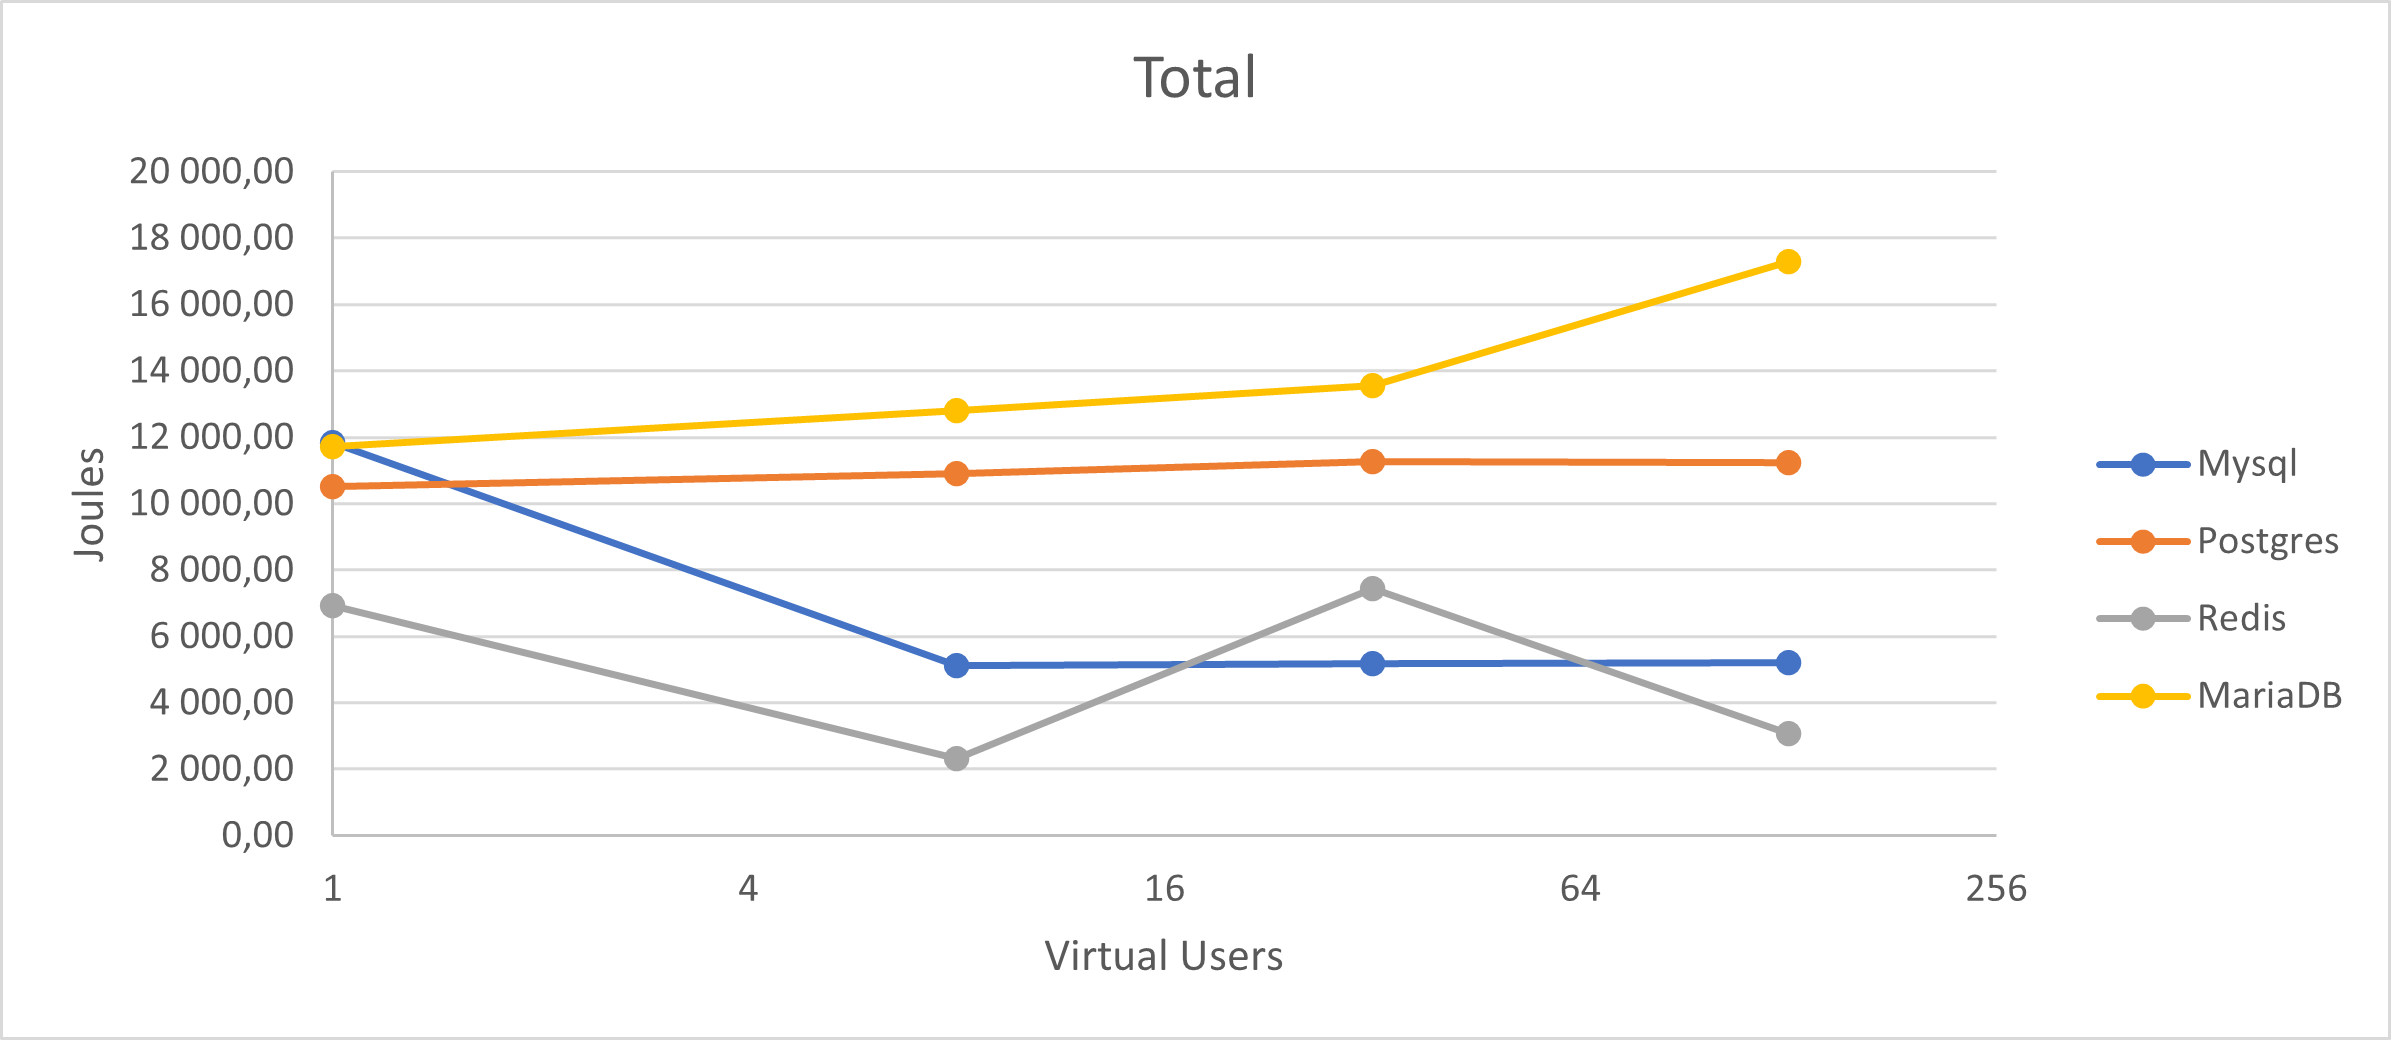
\includegraphics[width=0.76\columnwidth]{results/vu/Total.png}
\label{fig:vuyenergy}	
\end{figure*}
\begin{figure*}[h!]
\centering
\caption{Performance on HammerDB with different number of users.}
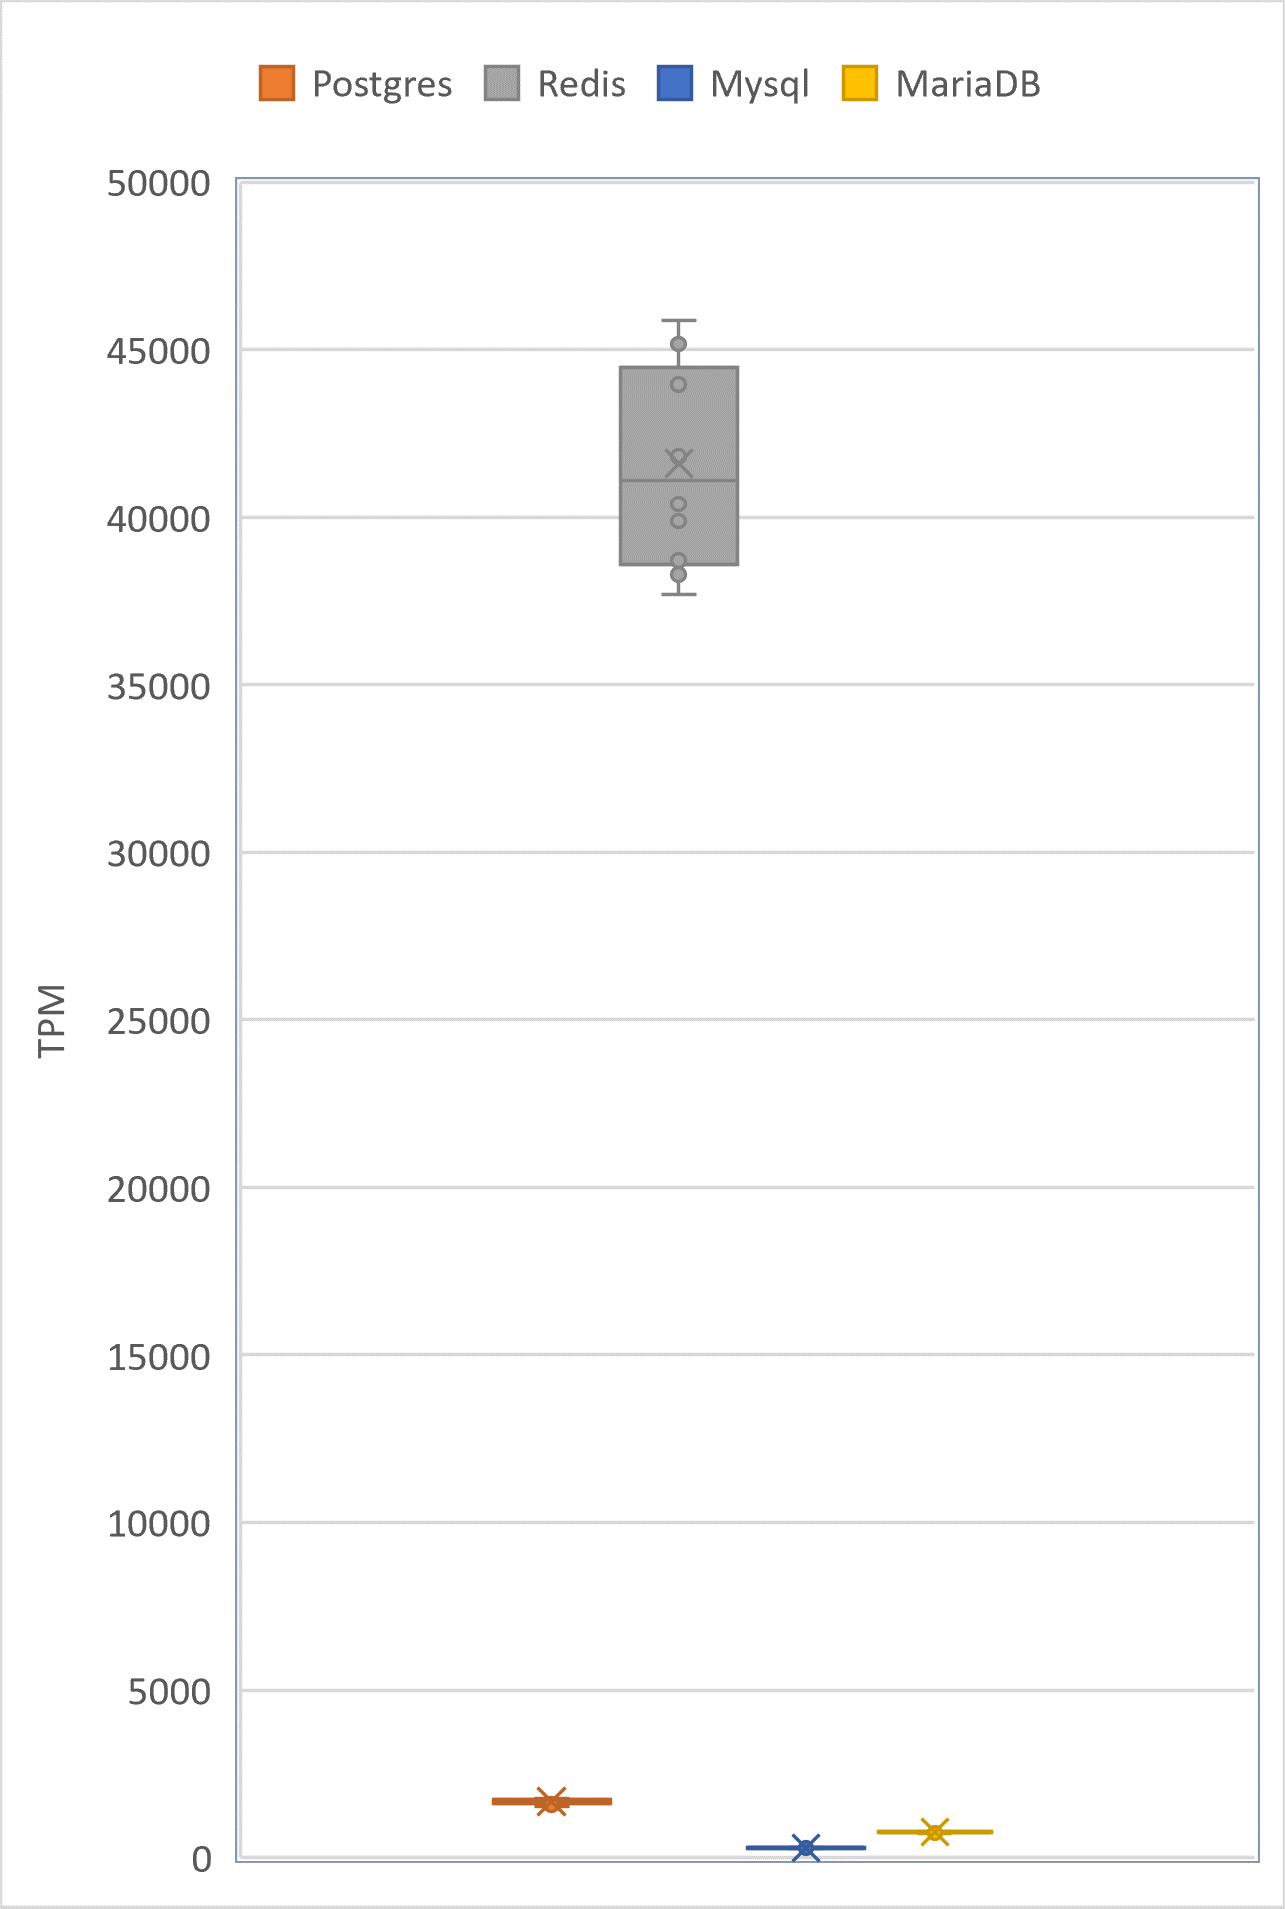
\includegraphics[width=0.76\columnwidth]{results/vu/TPM.png}
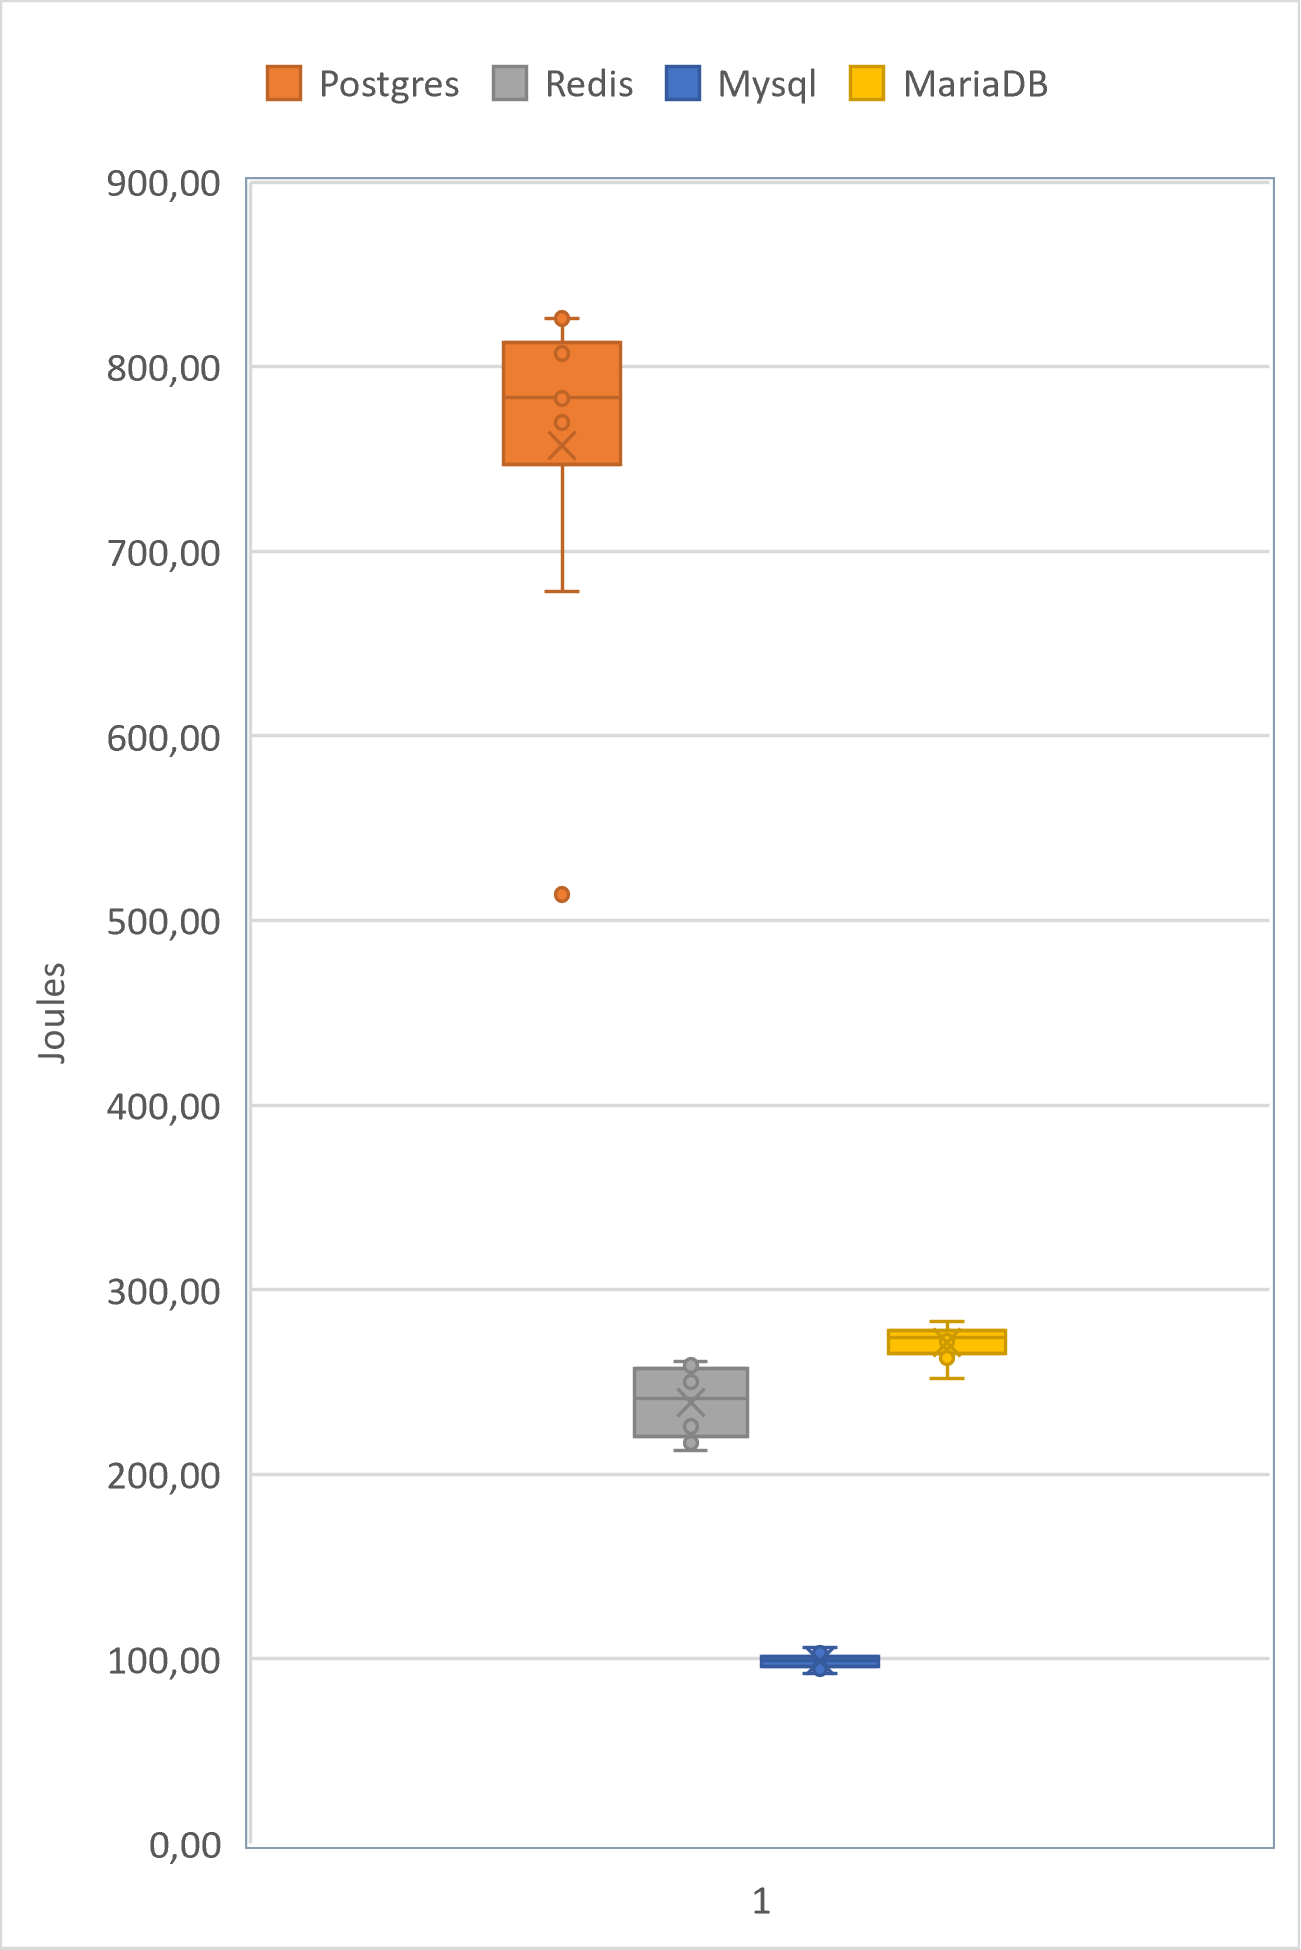
\includegraphics[width=0.76\columnwidth]{results/vu/NOPM.png}
\label{fig:vuhammer}	
\end{figure*}

\begin{figure*}[h!]
\centering
\caption{Energy consumption per Transitions per minute with different number of users.}
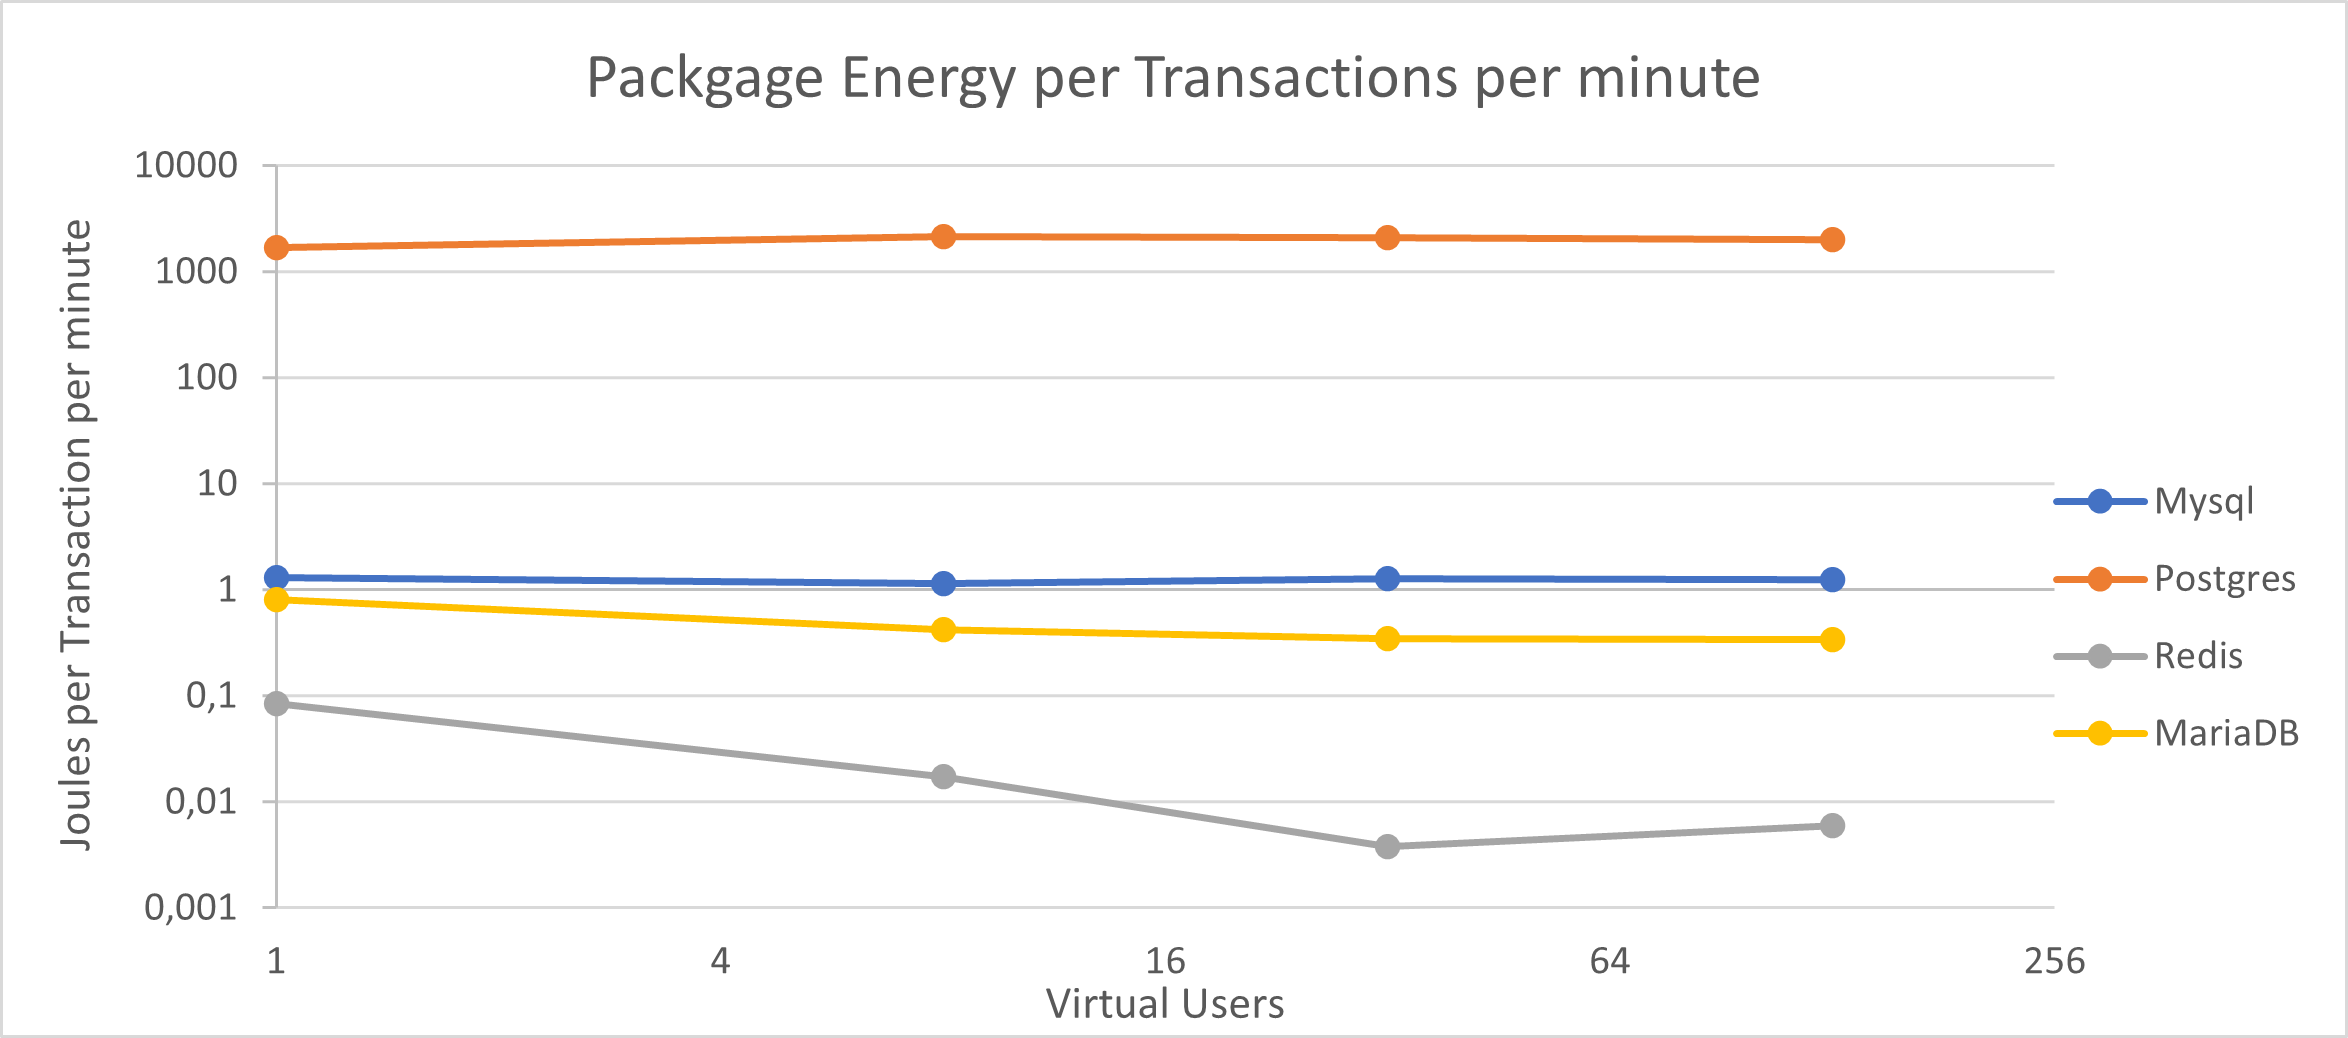
\includegraphics[width=0.76\columnwidth]{results/vu/package-tpm.png}
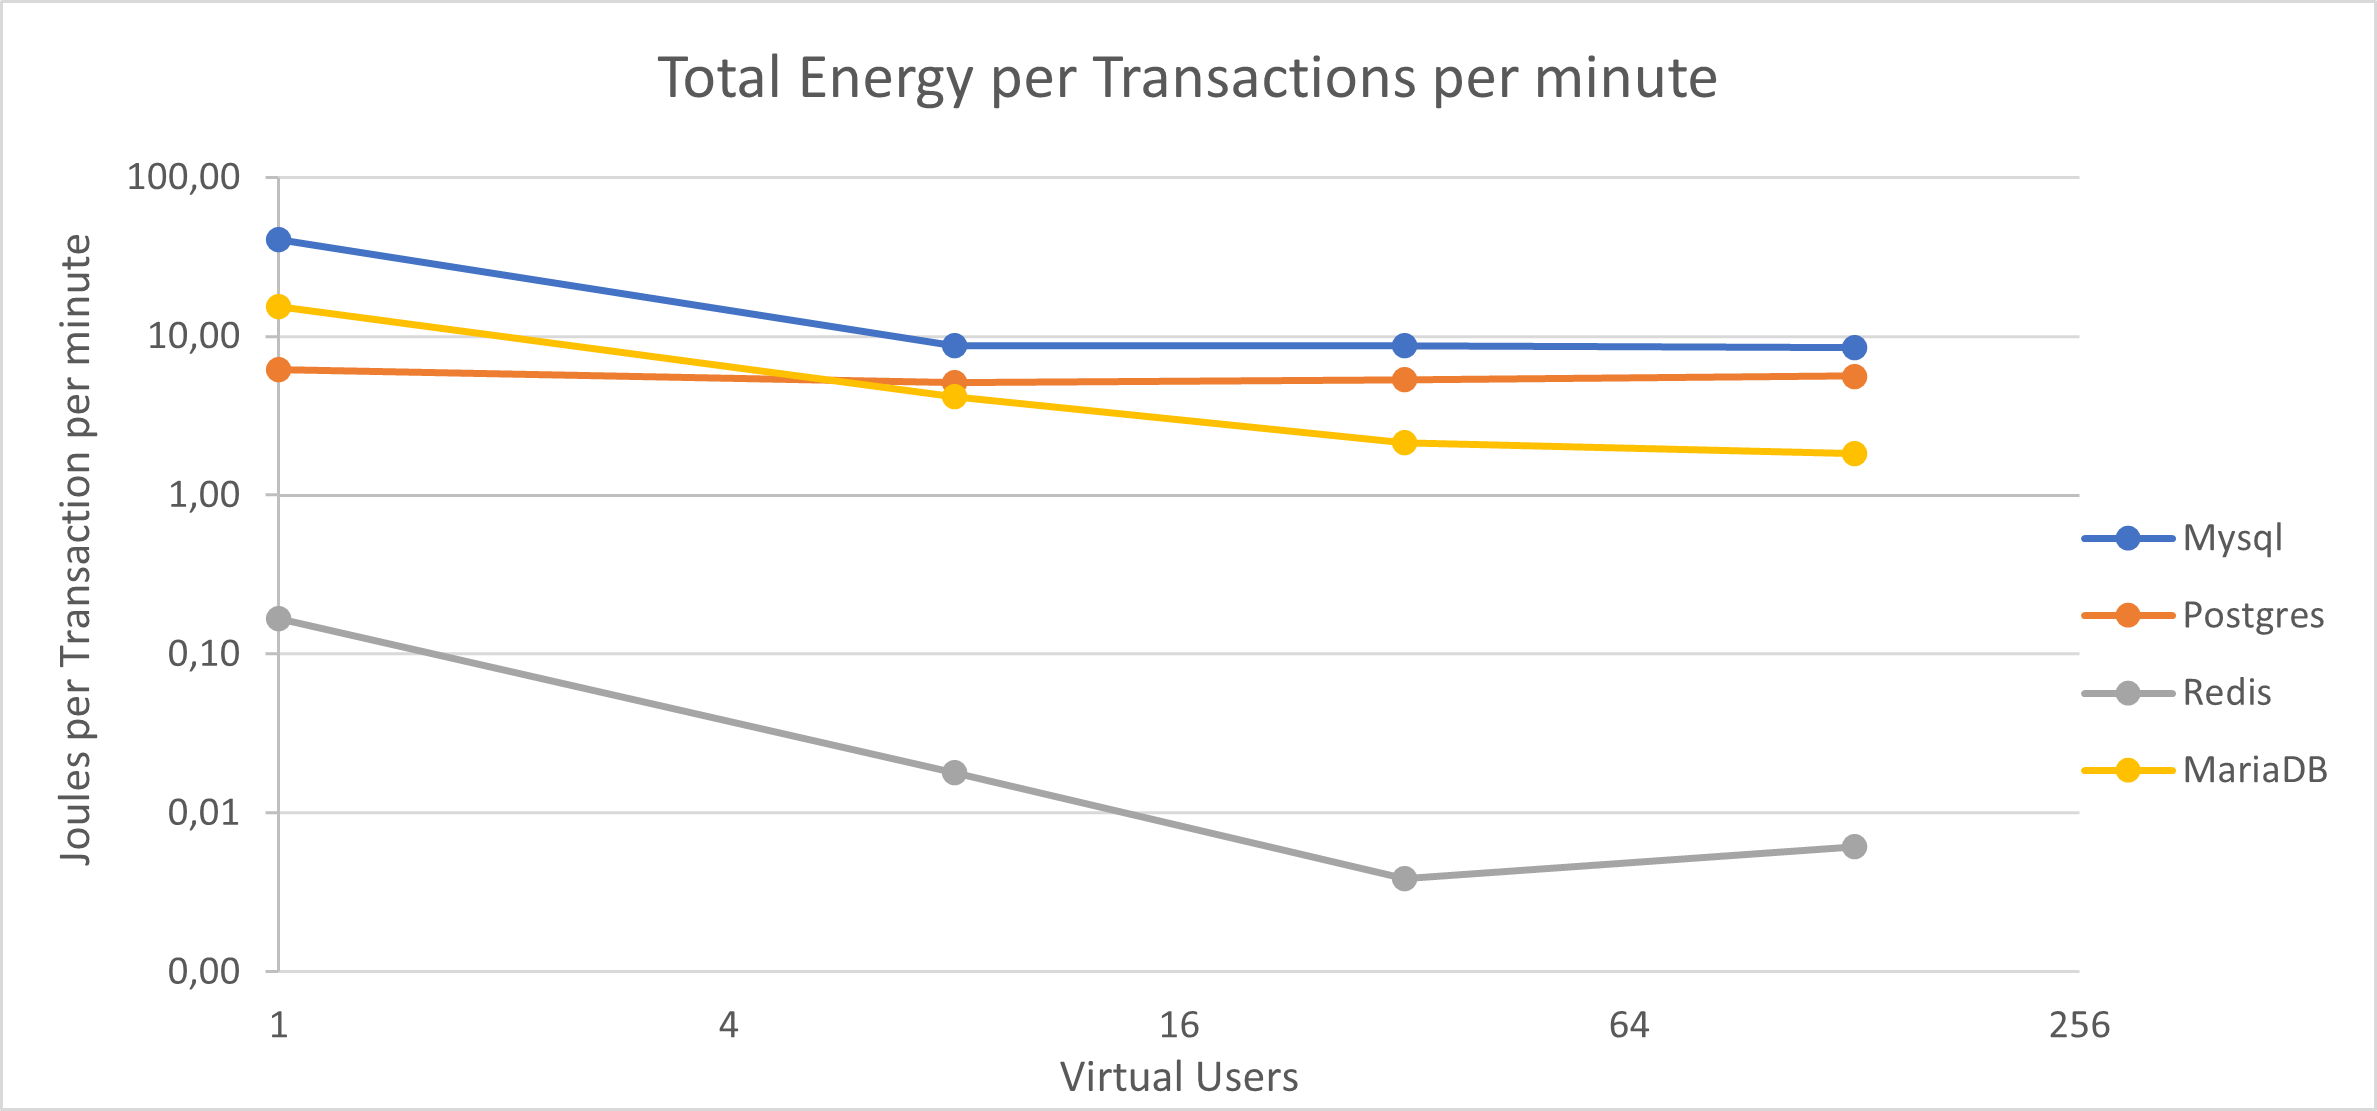
\includegraphics[width=0.76\columnwidth]{results/vu/total-tpm.png}
\includegraphics[width=0.76\columnwidth]{results/vu/Disk-tpm.png}
\label{fig:vuyenergytpm}	
\end{figure*}

\begin{figure*}[h!]
\centering
\caption{Energy consumption per Number of new orders with different number of users.}
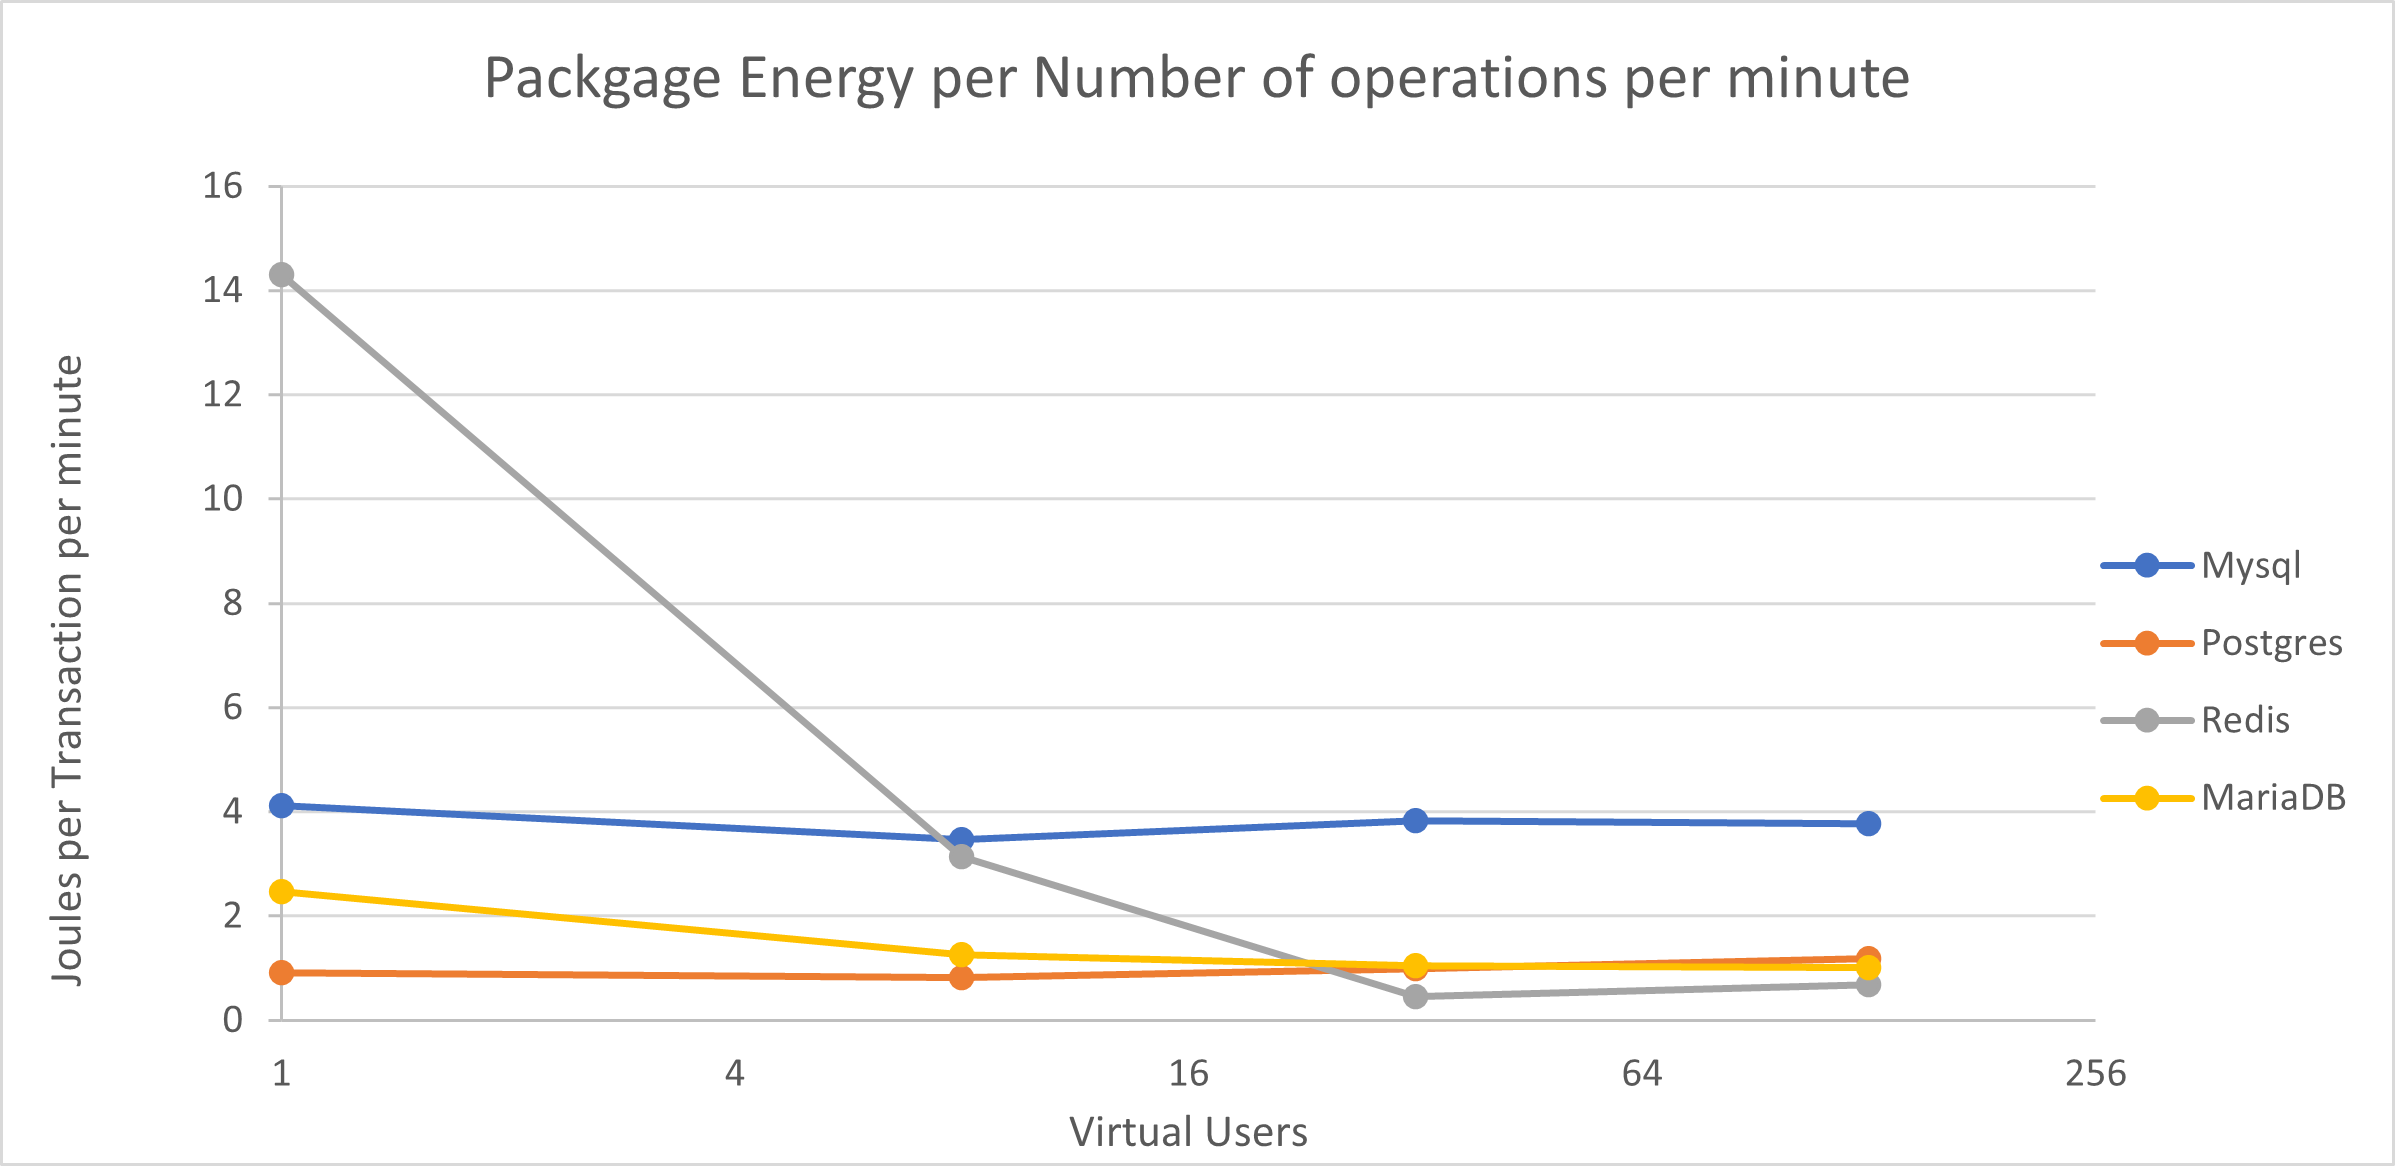
\includegraphics[width=0.76\columnwidth]{results/vu/Packgage-nopm.png}
\includegraphics[width=0.76\columnwidth]{results/vu/Disk-nopm.png}
\includegraphics[width=0.76\columnwidth]{results/vu/Total-nopm.png}
\label{fig:vuyenergynopm}	
\end{figure*}

For a better understanding of the results obtained from our study, we will display some graphical visualizations of the energy consumed by the different DMBS.

We all graphical visualizations, we decide not to focus and discuss the energy consumption on the RAM because values obtained were similar on every DBMS we put on the test. Also, we decide not to show in this paper the results of 10 minutes execution because it doesn't have a lot of difference between 5 minutes.

First, we focus on showing the results with only one user, for that we have bar graphs in Figure \ref{fig:medianenergy} showing the median amount of energy consumption each DBMS take at Package, CPU, Disk, and global system, we also made bar graphs for the hammerdb outputs (Transitions and New orders per minute) in Figure  \ref{fig:medianhammerdb}.

For a better understandable and detail of the previous results, we present in Figure \ref{fig:bocplotyenergy} the Box plot of the energy consumption of each DBMS and in Figure \ref{fig:bocplothammer} the output of the hammer DB. The box plot representation uses the median, the approximate quartiles, and the lowest and highest data points to convey the level, spread, and symmetry of a distribution of data values. It can also be easily refined to identify outlier data values and can be easily constructed by hand ~\cite{doi:10.7326/0003-4819-110-11-916}.  %referencia do box plot

With the graphs mention, we only can interpret and answer the \textit{RQ1}, for the \textit{RQ2}, to generate the transitions and Number of new orders per joules per minute, we had to divide the HAMMERDB  output for the energy, then we generate the same graphs mentions before but for this new values. We can see in Figure \ref{fig:medianenergyhammerdb} the median of the TPM per joules and the NOPM per joules for the Package, CPU, Disk, and global system. We also did the box plots for the same results, in the figure \ref{fig:bocplottrans} we can see the box plot for the  TPM per joules and in the figure \ref{fig:bocplotnumber} the box plot for the number operations per energy spent per minute and both of them for Package, Disk and global amount.

Finally, for the \textit{RQ3}, we did the figure \ref{fig:vuyenergy} that show the evolution of energy consumption(Y-axis) on Package, CPU, Disk and global system with the different numbers of virtual users (X-axis), the figure \ref{fig:vuhammer} shows the evolution of the performance of the hammerdb output with the different number virtual users and the figures \ref{fig:vuyenergytpm} and \ref{fig:vuyenergynopm}  shows the evolution of TPM and NOPM per joules with the different users.

For a better visualization, we decide not to show some of the CPU graphs since they are very similar with the Package graphs.
%%\begin{figure}[H]
  %\caption{Measurement of the total consumed energy by all DBMS.}
%  \centering
 % 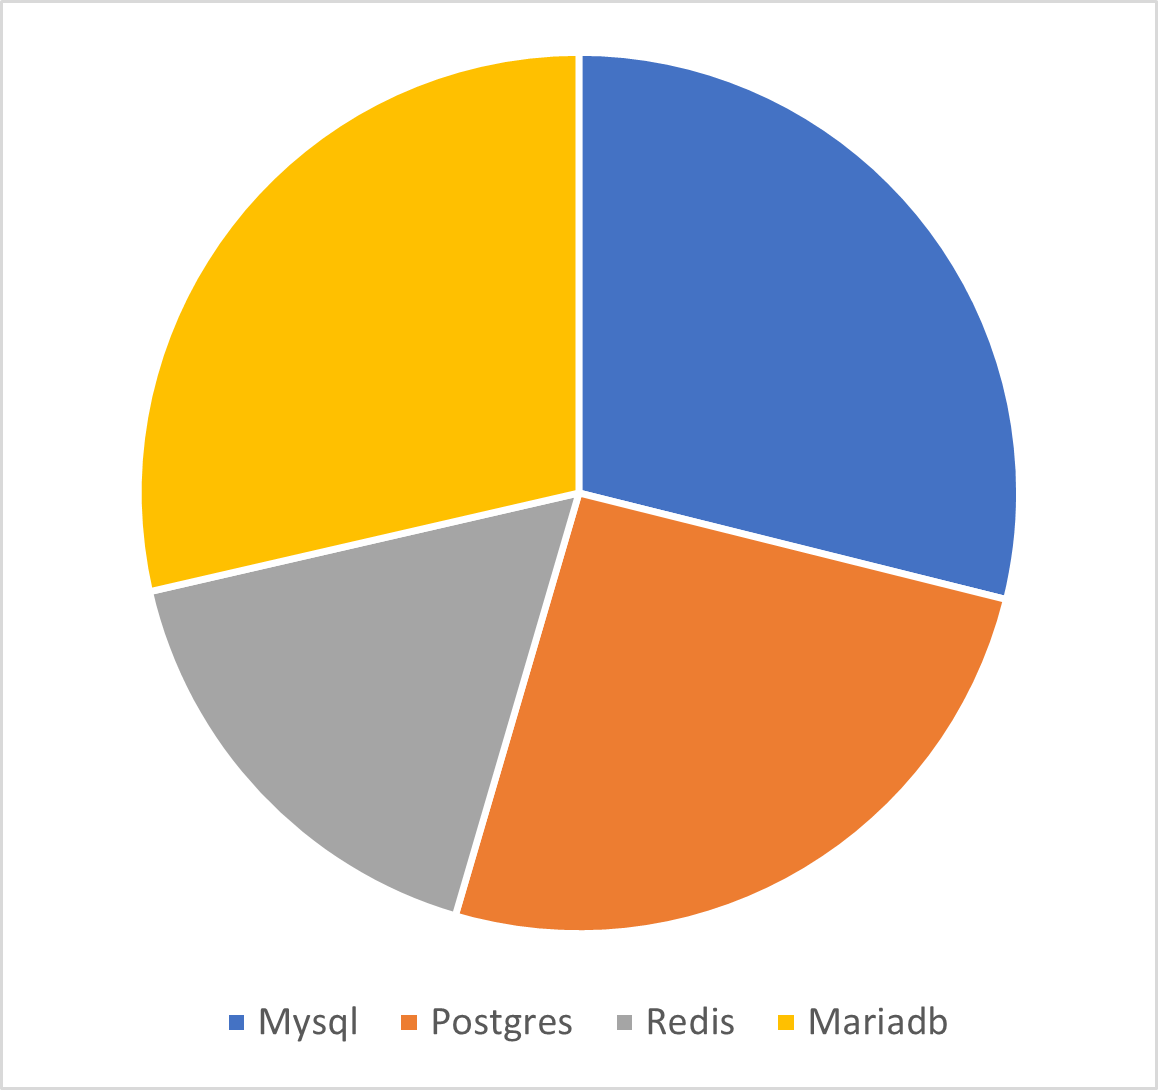
\includegraphics[width=0.7\linewidth]{results/piechart.png}
%  \label{fig:geraltotal}
%\end{figure}

\subsection{Discussion}


		We will discuss the results in order of the Research Question.
	    \subsubsection{RQ1}

	Beginning with the \textit{RQ1}, we will start talking about energy consumption on the Package level. As we can observe in figure \ref{fig:medianenergy}. Redis is the most consumption DBMS of the 4 DBMS follow by Postgres, MariaDB, and Mysql. We can see that all rational DBMS have energy consumption on the package very low comparing with the non-rational DBMS Redis.
	
	In terms of the distribution of the values, we can see in Figure \ref{fig:bocplotyenergy} that the distribution on the package level is very small on the relational databases, and only on Redis have a big distribution on the energy in the values. 
	
	On the Disk Level, as viewed in figure \ref{fig:medianenergy}, we can see the reverse of Package level happen, where the rational DBMS spending more energy and the non-rational consumption being the one that spent less. In this case, Mysql was the DBMS that spent more than MariaDB, Postgres, and Redis.
	
	On the disk, we can also see that there is almost no variation of results on the Redis and the same case scenario on the Postgres. But the distribution in MySQL and MariaDB is broad that while the median in MySQL is higher, some results are lower than the MariaDB median.
	
	In terms of total energy consumption even though Redis spent more than the others in the Package level, the energy he saves on the disk makes it the least expensive one, follow by MariaDB, Postgres, and Redis.  That happens because the secondary storage has a more significant overall impact on the total energy than the Package.
	
    \subsubsection{RQ2}

	
	Now with the \textit{RQ2}, As seen in Figure \ref{fig:medianhammerdb}, we can see that the non-relational DBMS Redis have a performance in terms of TPM, way better than the relational DBMS. We can also see that the ones with less consumption in the disk have a better performance overall. 
	
	In Terms of TPM per joules on the package, disk, and total, as seen in figure \ref{fig:medianenergyhammerdb}, it follows the same trend of the most expensive in terms of energy consumption where the Mysql is the most expensive followed by MariaDB, Postgres, and Redis. The distribution of these values in figure \ref{fig:bocplottrans} show that Mysql is always the most expensive followed by MariaDB, Postgres, and Redis.
	
	When talking about NOPM, as we can see in figure \ref{fig:medianenergyhammerdb} Postgres is the most with more new orders per minute, then MariaDB and Redis have the same number of NOPM and the lowest is Mysql. In terms of the distribution of these results, even though MariaDB and Redis have the same median Redis has a larger distribution as we can see in figure \ref{fig:bocplothammer}.
	
	In Terms of NOPM per joules, we can see the median in Figure \ref{fig:mediannopmenergy} that in the package the one with the most NOPM per Joules is Redis then Mysql, MariaDB, and Postgres. On the disk the one with the most NOPM per joules is Mysql then MariaDB, Redis, and finally Postgres. When talking of the system as a whole the Mysql is the one with the NOPM per joule, follow by MariaDB, Redis, and Postgres. This result doesn't follow any trend of the rational database being the most expensive or non relational database being the less expensive in any of the cases.

    \subsubsection{RQ3}
    
    First, we gonna analyze the energy consumption with the increase of the users as seen in Figure \ref{fig:vuyenergy}, in the package Redis, which have decreased with 8 users after that decrease have a large increase with 32 users follow by another decrease. The other databases have an increase in energy with the increase of the users.
    
    In the case of disk, MariaDB has an increase with the increase of users, Postgres also had an increase, MySQL has a decrease in energy, and Redis also had a decrease. And with these variations when we increase the number of users the MariaDB is the most expensive followed by Postgres, Mysql, and Redis.
    
    On a general view, Redis has the same pattern as in the disk being the lowest in terms of energy consumption except on 32 users, where the increase in Package has a large impact on the energy and putting in the second-lowest behind Mysql. Mysql with an increase of the users start to lower is energy consumption becoming the second-lowest energy consumption DBMS expect on 32 users where he is the lowest. The second highest is Postgres that have a small increase with the increase of users. Finally, MariaDB with the increase of users become the highest.   
    
    When we talk about the performance on the hammerdb benchmark as seen in figure \ref{fig:vuhammer}, first we can see all that bases had an increase of TPM and NOPM with an increase in the number of users. The only instance that had a decrease was from 32 to 128 users on Redis. With the increase of users, Redis still stay the Database with better TPM and NOPM and Mysql stays the worse, while Postgres with an increase of users start to get worse results comparing with MariaDB.
    
    When we talk about energy consumption per TPM as seen in Figure \ref{fig:vuyenergytpm}, we can see with the increase of users that Redis have a better "speed up" in terms of energy per TPM, in general, all the databases improve very well even though that MariaDB is the relational database with the better improves.
    
    Finally, in the Figure \ref{fig:vuyenergynopm} we can check the energy consumption per NOPM, We can see that all DBMS improve very well and we can see that Redis became the most efficient on energy consumption per NOPM with the increase of users, follow by MariaDB, Postgres, and Mysql.
    
    We can conclude that with the increase of virtual users that the nonrelational database Redis start to get better results on NOPM and TPM without a large increase in energy consumption making Redis the most scalable one. In terms of the Relational database, we saw that MariaDB had the most increase in hammerdb performance and in energy consumption per TPM and PM.
    